\documentclass[a4paper,UTF8,titlepage,10pt]{ctexart}
\CTEXsetup[format={\Large\bfseries}]{section}
\usepackage{amsmath}
\usepackage{caption}
\usepackage{graphicx}
\usepackage{float}
%\usepackage{epsfig}
%\usepackage{subfig}
\usepackage{subfigure}
%\usepackage{subcaption}
\usepackage{diagbox}
\def\pgfsysdriver{pgfsys-dvipdfmx.def}
\usepackage{tikz}
\usepackage{hyperref}
\usepackage{amsfonts,amssymb}
\usepackage{blindtext}
\usepackage[T1]{fontenc}
\usepackage[utf8]{inputenc}
\usepackage{listings}
\usepackage{afterpage}
\usepackage{pdfpages}
\usepackage{color}

\newcommand\myemptypage{
\null
\thispagestyle{empty}
\addtocounter{page}{-1}
\newpage}

\numberwithin{equation}{subsection}

\renewcommand\appendix{\par
	\setcounter{section}{0}
	\setcounter{subsection}{0}
	\gdef\thesection{附录 \Alph{section}}}


% 用来设置附录中代码的样式

\lstset{
	basicstyle          =   \sffamily,          % 基本代码风格
	keywordstyle        =   \bfseries,          % 关键字风格
	commentstyle        =   \rmfamily\itshape,  % 注释的风格,斜体
	stringstyle         =   \ttfamily,  % 字符串风格
	flexiblecolumns,                % 别问为什么,加上这个
	numbers             =   left,   % 行号的位置在左边
	showspaces          =   false,  % 是否显示空格,显示了有点乱,所以不现实了
	numberstyle         =   \zihao{-5}\ttfamily,    % 行号的样式,小五号,tt等宽字体
	showstringspaces    =   false,
	captionpos          =   t,      % 这段代码的名字所呈现的位置,t指的是top上面
	frame               =   lrtb,   % 显示边框
}

\lstdefinestyle{Python}{
	language        =   Python, % 语言选Python
	basicstyle      =   \zihao{-5}\ttfamily,
	numberstyle     =   \zihao{-5}\ttfamily,
	keywordstyle    =   \color{blue},
	keywordstyle    =   [2] \color{teal},
	stringstyle     =   \color{magenta},
	commentstyle    =   \color{red}\ttfamily,
	breaklines      =   true,   % 自动换行,建议不要写太长的行
	columns         =   fixed,  % 如果不加这一句,字间距就不固定,很丑,必须加
	basewidth       =   0.5em,
}

\hypersetup{colorlinks=true,linkcolor=black}
\begin{document}

\iffalse	
\begin{center}
\fontsize{25}{30} \selectfont  {\textbf{湘潭大学毕业论文}}  \\ 
\end{center}
\vspace{2cm}

\begin{center}
	\makeatletter
	\newcommand\dlmu[2][4cm]{\hskip1pt\underline{\hb@xt@ #1{\hss#2\hss}}\hskip3pt}
	\makeatother
	\zihao{3}
	\textbf{
	\begin{tabular}{rl}
		&\makebox[4em][s]{题目:}	  \hspace{0.2cm}   	\dlmu[9cm]{带间断系数的弹性问题的有限元方法} 	\\[2cm]
		&\makebox[4em][s]{学院:}    \hspace{0.2cm}	\dlmu[9cm]{数学与计算科学学院} \\ 
		&\makebox[4em][s]{班级:}	\hspace{0.2cm}		\dlmu[9cm]{2019 信息与计算科学二班}      \\
		&\makebox[4em][s]{学号:}	\hspace{0.2cm}	\dlmu[9cm]{201905755601}   \\
		&\makebox[4em][s]{姓名:}	\hspace{0.2cm}	\dlmu[9cm]{唐小康}   \\
		&\makebox[4em][s]{指导教师:}	\hspace{0.2cm}	\dlmu[9cm]{王华}   \\
	\end{tabular}}
\end{center}
\vspace{8cm}
\begin{center}
	\makeatletter
	\newcommand\dlmu[2][4cm]{\hskip1pt\underline{\hb@xt@ #1{\hss#2\hss}}\hskip3pt}
	\makeatother
	\zihao{3}
	\textbf{
	\makebox[4em][s]{完成日期:}	\hspace{0.2cm}	\dlmu[6cm]{2023年5月}}
\end{center}
\fi

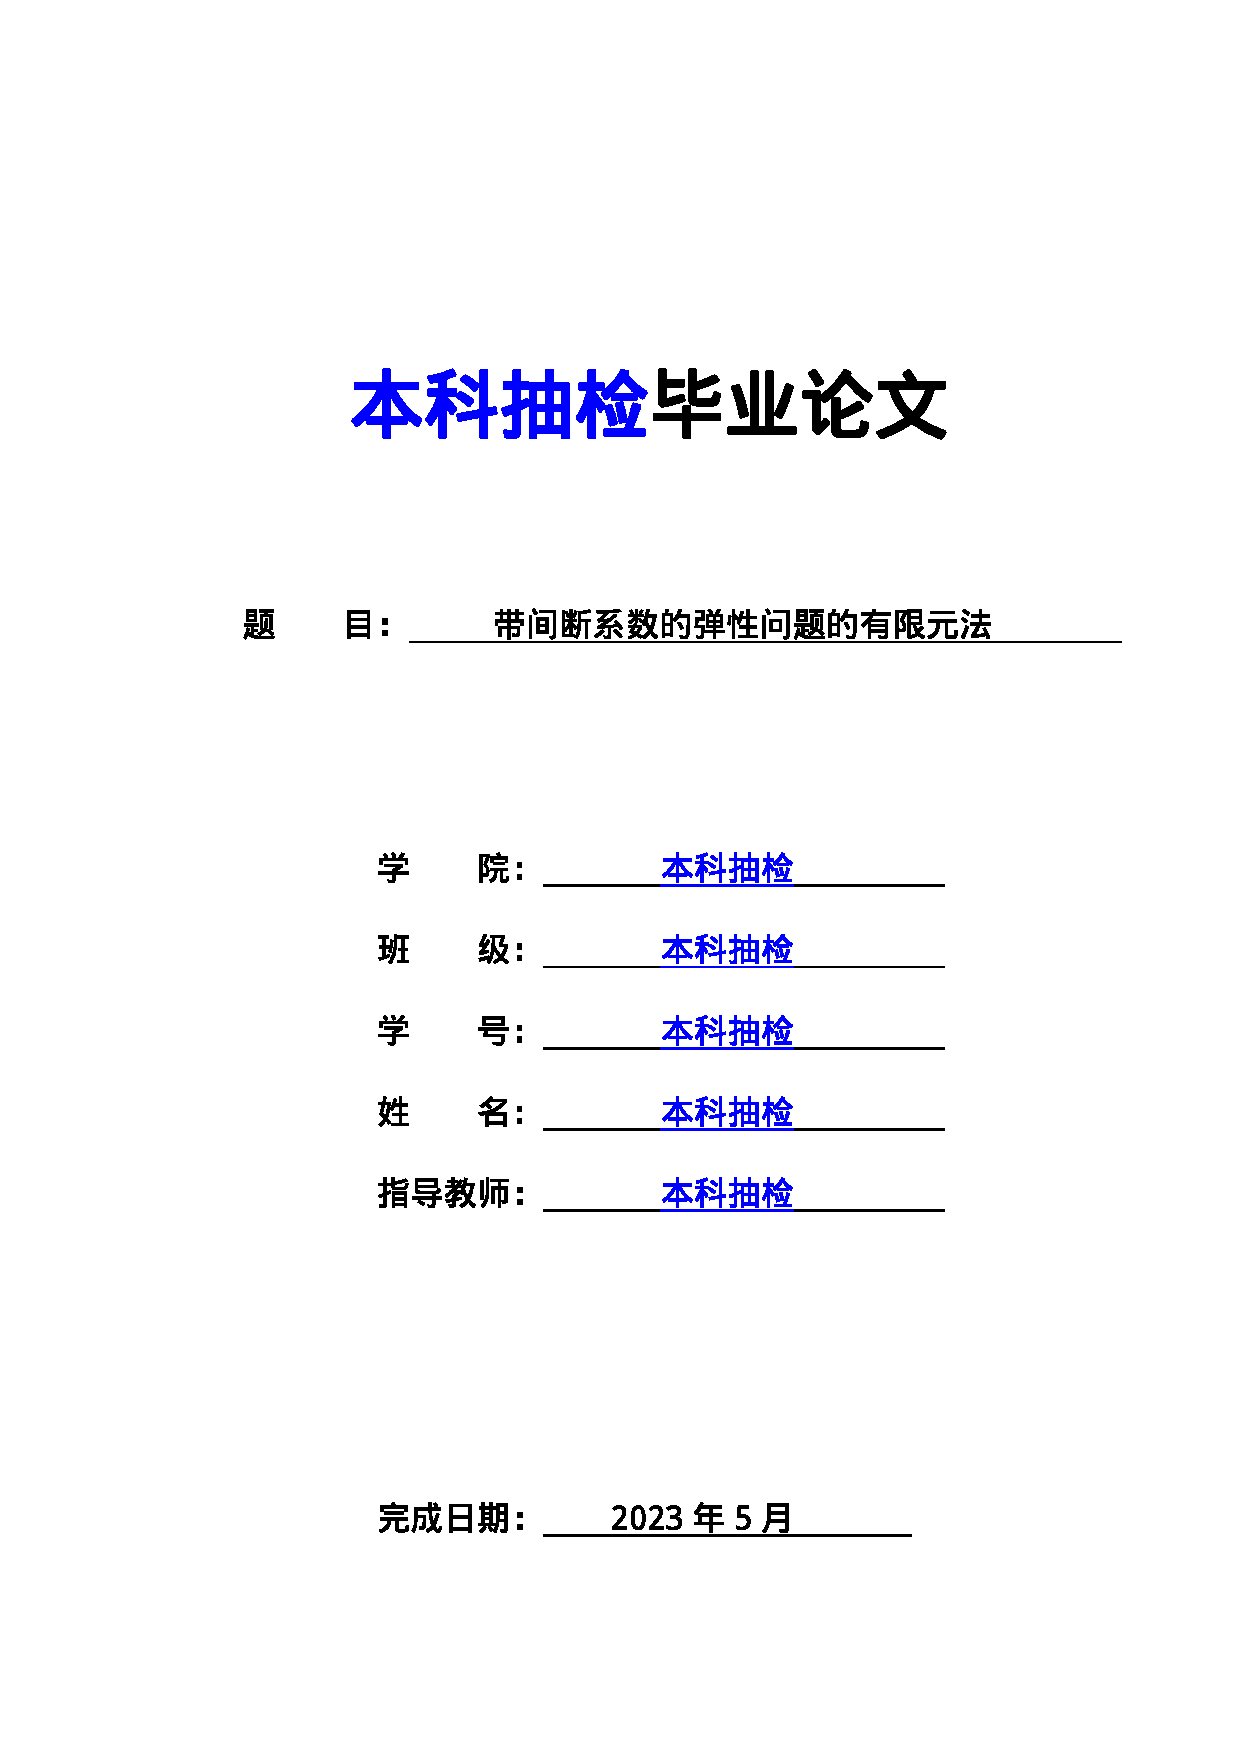
\includepdf[page={1}]{./push/终稿/匿名版/topdf.pdf}

\thispagestyle{empty}

%\title{带间断系数的弹性问题}
%\date{\today}
%\maketitle

\clearpage
\cleardoublepage

\pagestyle{plain}
\pagenumbering{Roman}
\renewcommand{\abstractname}{\vspace{-6cm}\large\bf 摘要}
\addcontentsline{toc}{section}{摘要}
\begin{abstract}
	
	本文以带间断系数的弹性问题为研究对象。首先介绍了研究背景和国内外研究现状,然后回顾了有限元理论的基本知识,包括Sobolev空间、弹性问题的边值问题和变分、带间断系数的方程的引入、离散方法和误差估计等。接着给出了几个算例,分别展示了弹性问题和带间断系数的弹性问题在有限元方法下的数值解,比较了不同的参数对结果的影响。最后总结了本文的主要结论,指出了存在的不足和未来的研究方向。  \\
	
	\noindent{\quad \quad \textbf{关键字:} 平面弹性问题; 间断系数;非协调有限元; locking-free}
\end{abstract}

\newpage
\newpage

\renewcommand{\abstractname}{\vspace{-6cm}\large Abstract}
\begin{abstract}
	
	This paper studies the elastic problem with discontinuous coefficients. Firstly, the research background and the domestic and foreign research status are introduced. Then, the basic knowledge of finite element theory is reviewed, including Sobolev space, boundary value problem and variational form of elastic problem, introduction of equation with discontinuous coefficients, discrete method and error estimation. Next, several examples are given to show the numerical solutions of elastic problem and elasticity problem with discontinuous coefficients under finite element method, and the influence of different parameters on the results is compared. Finally, the main conclusions of this paper are summarized, and the existing shortcomings and future research directions are pointed out.  \\
	
	\noindent{\quad \quad \textbf{Key words:} linear elasticity problem; discontinuous coefficient;nonconforming finite element; locking-free}
\end{abstract}
\addcontentsline{toc}{section}{Abstract}
%\thispagestyle{empty}

\newpage
\newpage

\tableofcontents
\thispagestyle{empty}

\newpage
\pagenumbering{arabic}

\section{绪论}

\subsection{研究背景}

带间断系数的方程是指一种用于模拟复合材料层合板的力学性能的数学模型。复合材料层合板是由两层或多层单层板粘合在一起的结构单元,具有不同的铺层顺序和铺层角度,可以表现出不同的力学特性。带间断系数的方程是一种考虑了层间应力和层间变形协调的方程,可以描述层合板在面内和面外的应力-位移关系。带间断系数的方程也可以用于模拟材料的分离和剥落,例如复合材料剥离、金属焊接材料损伤、混凝土材料开裂等。

平面弹性力学方程组是弹性力学中最基础、最常见的模型。当研究的弹性体形状和受力具有一定特点时,通过适当的简化处理,就可以归结为平面弹性问题 \textsuperscript{\cite{王兆清2018不可压缩平面问题的位移}}。
对于各向同性均匀介质的平面弹性问题,当材料的Lam$\acute{e}$常数$\lambda \to \infty$时,即对于几乎不可压介质,通常低阶的协调有限元解,往往不再收敛到原问题的解,或者达不到最优收敛阶,这就是闭锁现象\textsuperscript{\cite{陈绍春2007平面弹性的一个新的}}。

为了消除(近)不可压缩弹性问题中遇到的闭锁现象,国内外研究学者提出了多种有效的数值分析方法。根据型函数建立过程中是否需要网格剖分,这些数值方法可以分为两类:一类是有网格方法,这其中包括
高阶有限元法\textsuperscript{\cite{peet2014legendre}}、
混合有限元法\textsuperscript{\cite{masud2011variational}}、
增强有限元法\textsuperscript{\cite{auricchio2005analysis}}和
不连续Galerkin法\textsuperscript{\cite{hansbo2003discontinuous}}等;
另一类是无网格方法,无网格方法又可分为弱形式无网格法和强形式的无网格方法\textsuperscript{\cite{王兆清2018不可压缩平面问题的位移}}。

%本文将通过数值实验的方法,考察对于具有间断系数的平面弹性问题,使用C-R元是否仍可以解除闭锁现象。

\subsection{国内外研究现状}

有限元法是一种的数值分析方法,它可以用来求解各种复杂的工程问题。有限元法的核心思想最早可以追溯到 1943 年,当时 R.W.Courant 提出了一种基于变分原理的离散化方法。1956 年,R.W.Clough 等四位教授与工程师在一篇发表在科技期刊上的论文中,首次将这种方法应用到飞机机翼强度的计算中,并将其命名为刚性法(Stiffness)。这篇论文标志着有限元法在工程学界上的正式诞生。在 1960 年,R.W.Clough 教授在一篇关于平面弹性问题的论文中,首次提出了“有限元法”这个术语,并将这种方法应用到了土木工程领域。三年后,Richard MacNeal 博士与 Robert Schwendler 合作创立了 MSC 公司,并开发出了一款名为 SADSAM 的软件程序,实现了数字仿真模拟结构分析的功能,这标志着有限元方法 (FEA) 从理论走向了实践。1964-1965 年期间,O.C.Zienkiewicz 等人在多篇论文中,采用极小位能原理和虚功原理,以一种新颖的思路推导出了有限元法。

在我国,有限元方法的发展历史上,涌现出了一批杰出的学者,他们为有限元方法的理论和应用做出了重要的贡献,如冯康(有限单元法理论),陈伯屏(结构矩阵方法),钱令希(余能定理),钱伟长(广义变分原理)等。但是,受到当时的国际和国内环境的制约,我国的学者在有限元方法的深层次研究上遇到了很多困难,很难跟上国际的发展步伐,导致与国外的技术水平之间的差距逐步扩大。20世纪60年代初期,我国的老一辈计算科学家较早地将计算机应用于土木、建筑和机械工程领域。当时黄玉珊教授就提出了“小展弦比机翼薄壁结构的直接设计法”和“力法-应力设计法”;而在70年代初期,钱令希教授提出了“结构力学中的最优化设计理论与方法的近代发展”。这些理论和方法都为国内的有限元技术指明了方向。
1964年初崔俊芝院士研制出国内第一个平面问题通用有限元程序,解决了刘家峡大坝的复杂应力分析问题。20世纪60年代到70年代,国内的有限元方法及有限元软件诞生之后,曾计算过数十个大型工程,应用于水利、电力、机械、航空、建筑等多个领域。
20世纪70年代中期,大连理工大学研制出了JEFIX有限元软件,航空工业部研制了HAJIF系列程序。80年代中期,北京大学的袁明武教授通过对国外SAP软件的移植和重大改造,研制出了SAP-84;北京农业大学的李明瑞教授研发了FEM软件;建筑科学研究院在国家“六五”攻关项目支持下,研制完成了“BDP-建筑工程设计软件包”;中国科学院开发了FEPS、SEFEM;航空工业总公司飞机结构多约束优化设计系统YIDOYU等一批自主程序。

然而,在上世纪 90 年代,国外的有限元软件大规模地进入国内市场,涵盖了各个领域。国外的学者专家也经常到各大学、工厂和企业进行技术推广和使用指导,使得国内有限元方法的发展面临着更大的挑战。管理部门对有限元软件的认识也出现了偏差,对此缺少必要的支持,核心技术控制在国外,所以一直到上世纪末期,国内自主技术创新的速度十分缓慢。但是,在 21 世纪初期以来,国内拥有自主知识产权的软件逐渐实现了市场化,取得了一定的发展空间,同时也引起了国家对有限元技术的高度重视,使得有限元方法逐渐走出低迷状态,不再仅仅停留在高校和企业之中。

\newpage

\section{有限元理论}

\subsection{Sobolev空间}

假定 $G$ 是有界平面区域,其边界 $\Gamma$ 是按段光滑的简单闭曲线,$\overline{G} = G \cup \Gamma$ 是 $G$ 的闭包。对于 $\overline{G}$ 上的任一函数 $u(x,y),$ 称集合$\{(x,y) \, | \, u(x,y) \ne 0, \, (x,y) \in \overline{G}\}$ 的闭包为 $u$ 的支集。如果 $u$ 的支集 $\in G$ 内,则说 $u$ 于 $G$ 具有紧致支集。具有紧致支集的函数必在边界 $\Gamma$ 的某一邻域内恒等于零\textsuperscript{\cite{李荣华2007偏微分方程数值解}}。

用 $C_0^{\infty} $ 表示 $G$ 上无穷次可微并具有紧致支集的函数类,$L^2(G)$ 是定义在 $G$ 上平方可积的可测函数空间,其内积和范数分别为

\begin{equation}
	(f,g) = \int_G fg dxdy,
\end{equation}
\begin{equation}
	||f || = \sqrt{(f,f)} = (\int_G |f|^2 dxdy)^{\frac{1}{2}}.
\end{equation}

对 $f \in L^2(G),$ 如果存在$g,h \in L^2(G),$ 使等式

\begin{equation}
	\int_G g \varphi dxdy = - \int_g f \frac{\partial \varphi}{\partial x} dxdy ,
\end{equation}
\begin{equation}
	\int_G h \varphi dxdy = - \int_G f \frac{\partial \varphi}{\partial y} dxdy ,
\end{equation}

对任意的 $\varphi \in C_0^{\infty}$ 成立,则说 $f$ 对 $x$ 的一阶广义导数 $g$ 和对 $y$ 的一阶导数 $h,$ 记作

\begin{equation}
	f_x = \frac{\partial f}{\partial x} = g ,
\end{equation}
\begin{equation}
	f_y = \frac{\partial f}{\partial y} = y .
\end{equation}

定义 
$$
	H^1(G) = \{f(x,y) | f, f_x, f_y \in L^2(G) \} ,
$$
其中 $f_x, f_y $ 是 $f$ 的广义导数。与 $H^1(G)$ 引入内积
\begin{equation}
	(f,g)_1 = \int_G [fg + f_x g_x + f_y g_y] dxdy ,
\end{equation}
和范数
\begin{equation}
	||f||_1 = \sqrt{(f,f)} = (\int_G [|f|^2 + |f_x|^2 + |f_y|^2] dxdy )^{\frac{1}{2}} .
\end{equation}

则 $H^1(\Omega)$ 是 Hilbert 空间,称之为 Sobolev 空间。

\subsection{弹性问题}

\subsubsection{边值问题}

令$u$,$g$,$t$,$\sigma=(\sigma_{ij})_{1 \le i,j \le 2}$, $\tau = (\tau_{ij})_{1\le i,j \le 2}$ 是双变量函数,定义以下符号
$$
\begin{matrix}
	\epsilon(u) = \frac{1}{2} (grad \, u + (grad \, u)^t) , \\
	tr(\tau) = \tau_{11} + \tau_{22} , \\
	grad(u) = \begin{pmatrix}
		\frac{\partial u_1}{\partial x} & \frac{\partial u_1}{\partial y} \\
		\frac{\partial u_2}{\partial x} &
		\frac{\partial u_2}{\partial y}
	\end{pmatrix} , \\
	\delta = \begin{pmatrix}
		1 & 0 \\
		0 & 1
	\end{pmatrix} , \\
	div \, u = \frac{\partial u_1}{\partial x} + \frac{\partial u_2}{\partial y} , \\
	div \, \tau = \begin{pmatrix}
		\frac{\partial \tau_{11}}{\partial x} + \frac{\partial \tau_{12}}{\partial y} \\
		\frac{\partial \tau_{12}}{\partial x} + \frac{\partial \tau_{22}}{\partial 
			y} 
	\end{pmatrix} , \\
	\sigma : \tau = \sum\limits_{i=1}^{2} \sum\limits_{j=1}^{2} \sigma_{ij} \tau_{ij} .
\end{matrix}
$$

考虑各项同性弹性材料,令$u(x,y),f(x,y)$是其位移和体力,由线弹性问题的静态理论,$u,f$满足以下方程

\begin{equation}
\begin{aligned}
	-div \, \sigma(u) = f \quad  \in \Omega 
	%(\sigma(u) \nu) |_{\Gamma2} = t
\end{aligned}
\label{elasiticityEq} ,
\end{equation}

应力张量 $\sigma(u)$ 定义为
\begin{equation}
\sigma(u) = 2 \mu \epsilon(u) + \lambda tr(\epsilon(u)) \delta .
\end{equation}

其中 $\Omega \in \mathbb{R}^2,$ 正常数$\lambda, \, \mu$为 Lam$\acute{e}$ 常数。假定$(\mu, \lambda) \in [\mu_1,\mu_2] \times (0, +\infty).$

令 $\Gamma_1$、$\Gamma_2$ 为 $\partial \Omega$ 的两个开子集,使得 $\partial \Omega = \overline{\Gamma_1} \bigcup \overline{\Gamma_2}$ 并且 $\overline{\Gamma_1} \bigcap \overline{\Gamma_2} = \emptyset,$ 令$\Gamma_1$上的位移边界条件为
\begin{equation}
	u|_{\Gamma_1} = g .
\end{equation}
并且$\Gamma_2$上的牵引力边值条件为
\begin{equation}
	(\sigma(u) \nu) |_{\Gamma_2} = t .
\end{equation}

如果$\Gamma_1 = \emptyset \, (\mbox{或} \Gamma_2 = \emptyset),$ 则边值问题为纯牵引力(或纯位移)问题。

\subsubsection{变分}

对于齐次纯位移问题,令 $u$ 在边界上满足
\begin{equation}
u |_{\partial \Omega} = 0 .
\label{qcbjtj}
\end{equation}

设 $\nu = (\nu_1,\nu_2)^t, \, \nu_1, \nu_2 \in C_0^{\infty}(\Omega),$ 方程 $\eqref{elasiticityEq}$ 两边同乘 $\nu$ 并积分得

\begin{equation}
-\int_{\Omega} (div \, \sigma(u)) \, \nu \, dxdy = \int_{\Omega} f \nu \, dxdy .
\label{dycjf}
\end{equation}

参考文献知\textsuperscript{\cite{陈纪修2004数学分析}}

\begin{equation}
	f div \, a = div \, (fa) - a : grad \, f ,
\label{fbjf}
\end{equation}
\begin{equation}
	\int_{\Omega} div \, a \, dV = \int_{\partial \Omega} a \, dS .
\label{sddl}
\end{equation}

将边界条件$\eqref{qcbjtj}$,方程$\eqref{fbjf}$,$\eqref{sddl}$带入方程$\eqref{dycjf}$得

\par \quad \quad
$-\int_{\Omega} (div \, \sigma(u)) \, \nu \, dxdy$
$$ 
\quad \quad
\begin{matrix}
	\begin{aligned}
		&= -\int_{\Omega} div \, (\sigma(u) \nu) \, dxdy - \int_{\Omega} \sigma(u) : grad \, \nu \, dxdy \\
		&= -\int_{\Gamma} \sigma(u) \nu \, dxdy + \int_{\Omega} \sigma(u) : grad \, \nu \, dxdy \\
		&= \int_{\Omega} \sigma(u) : grad \, \nu \, dxdy \\
		&= \int_{\Omega} 2 \mu \epsilon(u) : grad \, \nu + \lambda \, div \, u \, div \, \nu \, dxdy  \\
		&= \mu \int_{\Omega} grad \, u : grad \, \nu \, dxdy + (\mu +\lambda) \int_{\Omega} div \, u \, div \, \nu \,  dxdy .
	\end{aligned}
\end{matrix}
$$

所以

\begin{equation}
\mu \int_{\Omega} grad \, u : grad \, \nu \, dxdy + (\mu +\lambda) \int_{\Omega} div \, u \, div \, \nu \, dxdy = \int_{\Omega} f \nu \, dxdy .
\end{equation}

\textbf{该问题的变分问题为},求$u \in H^1(\Omega)$ 使得 $u |_{\Gamma_1} = 0,$ 并且
\begin{equation}
a(u,\nu) = \int_{\Omega} f \cdot \nu \, dxdy \quad \forall \nu \in V ,
\label{bffc}
\end{equation}
\par
其中

\begin{equation}
	\begin{aligned}
		a(u,\nu) :&= \mu \int_{\Omega} grad \, u : grad \, \nu \, dxdy + (\mu +\lambda) \int_{\Omega} div \, u \, div \, \nu \,  dxdy , \\  		
		V :&= \{ \nu \in H^1(\Omega) \quad | \quad \nu |_{\Gamma} = 0 \} .
	\end{aligned}
\end{equation}

\textbf{Lax-Milgram定理\textsuperscript{\cite{brenner2008mathematical}}:} 设 $H$ 是 Hilbert 空间,$a(\cdot,\cdot)$ 是 $H \times H$ 上的有界的强制的双线性泛函。则对任意的$F \in H,$ 存在唯一的 $u \in H$ 满足
\begin{equation}
	a(u,\nu) = (f,\nu), \quad \forall \nu \in H .
\end{equation}

由Lax-Milgram定理知,此变分问题的解存在且唯一。

%证其与原问题的等价性

%\begin{enumerate}
%	\item 若 u 为原问题的解 \\


%	\item 若 u 为变分问题的解 \\
%	由
%	\par \quad \quad
%	$\int_{\Omega} \sigma(u) : grad \nu dxdy$
%	$$
%	\quad \quad
%	\begin{matrix}
	%		\begin{aligned}
		%			&= -\int_{\Gamma} \sigma(u) \nu dxdy + \int_{\Omega} \sigma(u) : grad %\nu dxdy \\
		%			&= -\int_{\Omega} div \sigma(u) \nu dxdy
		%		\end{aligned}
	%	\end{matrix} 
%	$$
%
%	得
%	$$
%		-\int_{\Omega} div \sigma(u) \nu dxdy = \int_{\Omega} f \nu dxdy
%	$$
%	
%	由变分法基本引理得
%	$$
%		-div \sigma(u) = f
%	$$
%	
%\end{enumerate}

\subsubsection{引入间断系数}

设 $\Omega_1$,$\Omega_2$ 是 $\Omega$ 的两个子集,使得 $\Omega_1 \bigcup \Omega_2 = \Omega$ 并且 $\Omega_1 \bigcap \Omega_2 = \emptyset,$

考虑以下边值问题
\begin{equation}
\begin{aligned}
	-div \, \sigma(u) &= f \quad \in \Omega, \\
	u |_{\partial \Omega} &= 0 .
\end{aligned}
\end{equation}

当Lam$\acute{e}$ 常数 $\lambda, \, \mu$ 在 $\Omega_1, \, \Omega_2$ 上取不同值,即 $(x,y) \in \Omega_1$ 时 $\lambda = \lambda_1, \, \mu = \mu_1 , \,(x,y) \in \Omega_2$ 时 $\lambda = \lambda_2, \, \mu = \mu_2,$ 并且 $\lambda_1 \ne \lambda_2, \, \mu_1 \ne \mu_2,$ 通过计算得到与此问题对应的双线性形式为
\begin{equation}
\begin{aligned}
	a(u,\nu) &= \mu_1 \int_{\Omega_1} grad \, u : grad \, \nu \, dxdy + (\mu_1 +\lambda_1) \int_{\Omega_1} div \, u \, div \, \nu \,  dxdy \\
	&+ \mu_2 \int_{\Omega_2} grad \, u : grad \, \nu \, dxdy + (\mu_2 +\lambda_2) \int_{\Omega_2} div \, u \, div \, \nu \, dxdy .
\end{aligned}
\end{equation}

\subsection{离散}

\subsubsection{Galerkin法}

\begin{figure}[h]
	\centering
	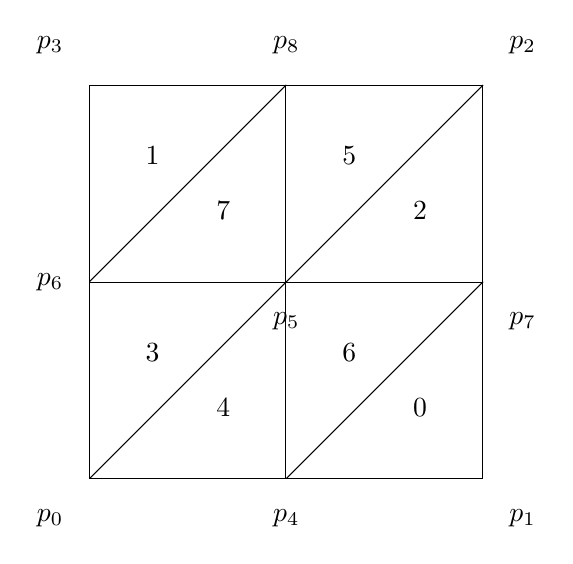
\begin{tikzpicture}
		\draw [step=71pt] (0,5) grid (5,0);
		
		\draw (0,0)--(5,5);
		\draw (0,2.5)--(2.5,5);
		\draw (2.5,0)--(5,2.5);
		
		\node at(-0.5,-0.5) {$p_0$};
		\node at(2.5,-0.5)  {$p_4$};
		\node at(5.5,-0.5)  {$p_1$};
		\node at(-0.5,2.5)  {$p_6$};
		\node at(2.5,2)     {$p_5$};
		\node at(5.5,2)     {$p_7$};
		\node at(-0.5,5.5)  {$p_3$};
		\node at(2.5,5.5)   {$p_8$};
		\node at(5.5,5.5)   {$p_2$};
		
		\node at(0.8,1.6) {3};
		\node at(1.7,0.9) {4};
		\node at(3.3,1.6) {6};
		\node at(4.2,0.9) {0};
		\node at(0.8,4.1) {1};
		\node at(1.7,3.4) {7};
		\node at(3.3,4.1) {5};
		\node at(4.2,3.4) {2};
	\end{tikzpicture}
	\caption{}
	\label{hf}
\end{figure}

设求解区间$\Omega = [0,1] \times [0,1],$ 首先对其按照图$\ref{hf}$进行网格剖分,节点为
$$
p_0, p_1, ... , p_n .
$$
图中的三角形区域称为单元。

其次,在Sobolev空间 $H^1$ 内取子空间 $U_h,$ 它的元素在每一单元是次数不超过某一正整数 $m$ 的多项式,在全区域 $\Omega$ 上属于函数空间 $H^1.$ 则 $U_h \times U_h$ 为试探函数空间。

设
$$
\begin{matrix}
	U_h = span(\varphi_0, \varphi_1, ... , \varphi_n) , \\
	\phi_{2i} = (\varphi_i, 0), \quad \phi_{2i+1} = (0, \varphi_i), \quad i=0,...,n .
\end{matrix}
$$

则 $\forall u_h \in U_h \times U_h,$ 可表成
\begin{equation}
	u_h = \sum\limits_{i=0}^{2n+1} c_i \phi_i .
	\label{uh}
\end{equation}

将式 $\eqref{uh}$ 带入方程 $\eqref{bffc}$中得到 Galerkin 方程
\begin{equation}
	\sum\limits_{i=0}^{2n+1} a(\phi_i, \phi_j) c_i = (f,\phi_j), \quad j = 0, 1, ... , 2n+1 .
	\label{galerkin}
\end{equation} 

令

$$
\begin{matrix}
	A = (a(\phi_j, \phi_i))_{0 \le i,j \le 2n+1} , \\
	F = ((f,\phi_i))_{0 \le i \le 2n+1} , \\
	c = (c_i)_{0 \le i \le 2n+1} .
\end{matrix}
$$

则 Galerkin 方程$\eqref{galerkin}$的矩阵形式为

\begin{equation}
	Ac = F .
\end{equation}

考虑齐次边界条件,若$(x_i,y_i)$为边界点,则 $A$ 第 $2i$ 行第 $2i$ 列,第 $2i+1$ 行第 $2i+1$ 列元素为$1,$第 $2i$ 和 $2i+1$ 行的其他元素及  $F(2i),F(2i+1)$ 都为 $0.$

\subsubsection{线性元}

如图$\ref{xxy}$,设 $ \bigtriangleup(p_0,p_1,p_2) $ 是以 $p_0,p_1,p_2$ 为顶点的任意三角型元,面积为 $S.$ 在 $ \bigtriangleup (p_0,p_1,p_2) $ 内任取一点 $p,$ 坐标为$(x,y).$ 过 $p$ 点作与三个顶点的连线,将 $ \bigtriangleup(p_0,p_1,p_2) $ 分成三个三角形: $ \bigtriangleup(p_1,p_2,p), \, \bigtriangleup(p_0,p,p_2), \, \bigtriangleup(p_0,p_1,p),$ 其面积分别为$S_0,S_1,S_2.$ \textsuperscript{\cite{李荣华2007偏微分方程数值解}}

%\begin{figure}[hbt]
%	\centering
%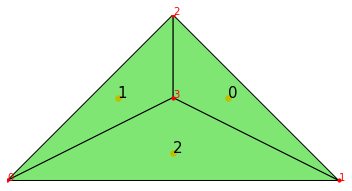
\includegraphics[height=3cm,width=4cm]{../image/TriangleElement.png}
%	\caption{}
%	\label{SampleOfDatasets}
%\end{figure}

\begin{figure}[h]
	\centering
	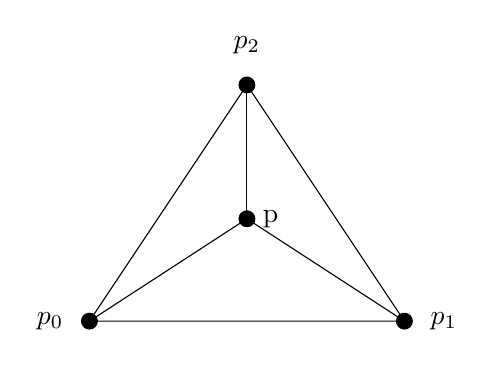
\begin{tikzpicture}
		\draw (3,0)--(7,0)--(5,3)--cycle;
		\draw (3,0)--(5,1.3)--(7,0);
		\draw (5,1.3)--(5,3);
		\filldraw (3,0)   circle(.1)
		(7,0) circle(.1)
		(5,3) circle(.1)
		(5,1.3) circle(.1);
		\node at(2.5,0)  {$p_0$};
		\node at(7.5,0)   {$p_1$};
		\node at(5,3.5)   {$p_2$};
		\node at(5.3,1.3) {p};
	\end{tikzpicture}
	\caption{}
	\label{xxy}
\end{figure}

显然$S_0 + S_1 + S_2 = S,$ 令
\begin{equation}
L_0 = \frac{S_0}{S}, \quad L_1 = \frac{S_1}{S}, \quad L_2 = \frac{S_2}{S} ,
\end{equation}
\par
%称$(L_0,L_1,L_2)$位$P_3$的面积坐标,其中
%$$
%	\begin{cases}
	%		2S = \left| \begin{matrix}
		%				1 & x_0 & y_0 \\
		%				1 & x_1 & y_1 \\
		%				1 & x_2 & y_2
		%			 \end{matrix} \right| ,
	%		 \quad
	%		 2S_0 = \left| \begin{matrix}
		%		 			1 & x   & y   \\
		%		 			1 & x_1 & y_1 \\
		%		 			1 & x_2 & y_2
		%		 \end{matrix} \right| 
	%		 \\
	%		2S_1 = \left| \begin{matrix}
		%					1 & x_0 & y_0 \\
		%					1 & x   & y   \\
		%					1 & x_2 & y_2
		%			   \end{matrix} \right|,
	%		\quad
	%		2S_2 = \left| \begin{matrix}
		%					1 & x_0 & y_0 \\
		%					1 & x_1 & y_1 \\
		%					1 & x   & y
		%			   \end{matrix} \right|
	%	\end{cases}
%$$

%由此可得面积坐标和直角坐标的转化关系
%$$
%\begin{cases}
%	x = x_0 L_0 + x_1 L_1 + x_2 L_2 \\
%	y = y_0 L_0 + y_1 L_1 + x_2 L_2
%\end{cases}
%$$
$$
\begin{cases}
	L_0 = \frac{1}{2S} [(x_2 y_3 - x_3 y_2) + (y_2 - y_3) x + (x_3 - x_2) y], \\
	L_1 = \frac{1}{2S} [(x_3 y_0 - x_0 y_3) + (y_3 - y_0) x + (x_0 - x_3) y], \\
	L_2 = \frac{1}{2S} [(x_0 y_1 - x_1 y_0) + (y_0 - y_1) x + (x_1 - x_0) y]. 
\end{cases} 
$$

因为

$$
\begin{cases}
	L_0 = \begin{cases}
		1, \quad x = x_0, y = y_0, \\
		0, \quad x = x_1, y = y_1, \\
		0, \quad x = x_2, y = y_2,
	\end{cases} \\
	L_1 = \begin{cases}
		0, \quad x = x_0, y = y_0, \\
		1, \quad x = x_1, y = y_1, \\
		0, \quad x = x_2, y = y_2,
	\end{cases} \\
	L_2 = \begin{cases}
		0, \quad x = x_0, y = y_0, \\
		0, \quad x = x_1, y = y_1, \\
		1, \quad x = x_2, y = y_2,
	\end{cases}  \\
\end{cases}
$$

所以在此区间上 $\varphi_i = L_i$,即

\begin{equation}
\begin{cases}
	\varphi_0 = \frac{1}{2S} [(x_2 y_3 - x_3 y_2) + (y_2 - y_3) x + (x_3 - x_2) y], \\
	\varphi_1 = \frac{1}{2S} [(x_3 y_0 - x_0 y_3) + (y_3 - y_0) x + (x_0 - x_3) y], \\
	\varphi_2 = \frac{1}{2S} [(x_0 y_1 - x_1 y_0) + (y_0 - y_1) x + (x_1 - x_0) y]. 
\end{cases} 
\end{equation}


\subsubsection{C-R元}

如图$\ref{CRElem}$, 设三角形 $\bigtriangleup(q_0,q_1,q_2)$ 是以 $q_0,q_1,q_2$ 为顶点的任意三角形元,$\, p_0,p_1,p_2$ 为其三条边的中点,其坐标分别为$(x_0.y_0),(x_1,y_1),(x_2,y_2).$

\begin{figure}[h]
	\centering
	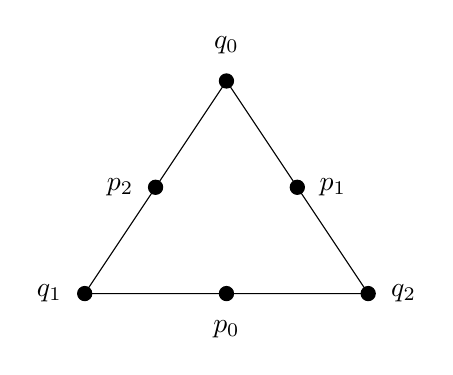
\begin{tikzpicture}[scale=0.9]
		\draw (0,0)--(4,0)--(2,3)--cycle;
		\filldraw (2,0)   circle(.1)
		(3,1.5) circle(.1)
		(1,1.5) circle(.1)
		(0,0) circle(.1)
		(4,0) circle(.1)
		(2,3) circle(.1);
		
		\node at(2,-0.5)  {$p_0$};
		\node at(3.5,1.5) {$p_1$};
		\node at(0.5,1.5) {$p_2$};
		
		\node at(-0.5,0) {$q_1$};
		\node at(4.5,0) {$q_2$};
		\node at(2,3.5) {$q_0$};
	\end{tikzpicture}
	\caption{}
	\label{CRElem}
\end{figure}

设三角形 $\bigtriangleup(q_0,q_1,q_2)$ 上的C-R元为 $\varphi_0, \varphi_1,\varphi_2,$

\begin{equation}
\varphi_i = a_i x + b_i y + c_i, \quad i = 0,1,2 ,
\end{equation}

且其在 $p_0$,$p_1$,$p_2$ 点上满足以下关系式

\begin{equation}
\varphi_i(p_j) = \begin{cases}
	1, \quad i = j \\
	0, \quad i \ne j	
\end{cases}, \quad i, j = 0,1,2 .
\label{crjs}
\end{equation}

设

$$
A = \begin{bmatrix}
	x_0 & y_0 &1 \\
	x_1 & y_1 &1 \\
	x_2 & y_2 &1 \\
\end{bmatrix}, \quad 
c_i = (a_i,b_i,c_i)^t , \quad
f = (x,y,1)^t .
$$

则方程组 $\eqref{crjs}$ 的矩阵形式为

\begin{equation}
A c_i = e_i, \quad i = 0,1,2 .
\end{equation}

通过计算可以得到单元$\bigtriangleup(q_0, q_1, q_2)$ 上的 C-R 元为

\begin{equation}
\varphi_i = A^{-1} e_i f, \quad i = 0,1,2 .
\end{equation} 

\iffalse
$$
\begin{cases}
	\begin{cases}
		\varphi_0(p_0) = a_0 x_0 + b_0 y_0 + c_0 = 1 \\
		\varphi_0(p_1) = a_0 x_1 + b_0 y_1 + c_0 = 0 \\
		\varphi_0(p_2) = a_0 x_2 + b_0 y_2 + c_0 = 0
	\end{cases} \\
	\begin{cases}
		\varphi_1(p_0) = a_1 x_0 + b_1 y_0 + c_1 = 0 \\
		\varphi_1(p_1) = a_1 x_1 + b_1 y_1 + c_1 = 1 \\
		\varphi_1(p_2) = a_1 x_2 + b_1 y_2 + c_1 = 0 
	\end{cases} \\
	\begin{cases}
		\varphi_2(p_0) = a_2 x_0 + b_2 y_0 + c_2 = 0 \\
		\varphi_2(p_1) = a_2 x_1 + b_2 y_1 + c_2 = 0 \\
		\varphi_2(p_2) = a_2 x_2 + b_2 y_2 + c_2 = 1
	\end{cases}
\end{cases}
$$
\fi

\subsection{误差估计}

假设$\Omega$是一个凸多边形区域,并且$\Gamma_1$ or $\Gamma_2$中任意一个为空。对于纯位移问题$(\Gamma_2=\emptyset),$ 只考虑齐次边界条件。
\par
令$T^h$ 是$\Omega$ 三角划分的一个非退化族。对于纯位移问题$(\Gamma_2=\emptyset),$ 使用有限元空间
% \begin{equation}\label{equ1} (\ref{newton})引用
	%	V_h := \{ \nu \in H^1(\Omega) : \nu |_{\emph{T}} \mbox{为线性函数}, \forall \emph{T} \in \emph{T}^h \}
	% \end{equation}
$$
V_h := \{ \nu \in H^1(\Omega) : \nu |_{T} , \, \forall T \in T^h \},
$$
并且对于纯牵引力问题$(\Gamma_1 = \emptyset),$ 使用
% \begin{equation}\label{equ2}
	%	V_h :=
	%\end{equation}
	$$
	V_h := \{ \nu \in H^1(\Omega) : \nu |_{T} , \, \forall T \in T^h \},
	$$
%	\\ \\
%	根据第二章和第四章的理论我们得到以下定理。
	令 $u \in H^2(\Omega) \cap H^1(\Omega)$ 满足纯位移问题,并且$u_h \in V_h$ 满足
	\begin{equation}
	a(u_h, \nu) = \int_{\Omega} f \cdot \nu \, dx \quad \forall \nu \in V_h.
	\end{equation}
	\\
	则存在一个正常数$C_{(\mu, \lambda)}$ 使得\textsuperscript{\cite{brenner2008mathematical}}
	\begin{equation}
	\quad \quad \quad
	\| u - u_h \|_{H^1(\Omega)} \le C_{(\mu, \lambda)} h \| u \|_{H^2(\Omega)}.
	\end{equation}
	令 $u \in H^2(\Omega)$ 满足纯牵引力问题。令 $u_h \in V_h$ 满足
	\begin{equation}
	a(u_h,\nu) = \int_{\Omega} f \cdot \nu \, dx + \int_{\Gamma_2} t \cdot \nu \, ds \quad \forall \nu \in V_h.
	\end{equation}
	\\
	则存在一个正常数$C_{(\mu, \lambda)}$ 使得\textsuperscript{\cite{brenner2008mathematical}}
	\begin{equation}
	\| u - u_h \|_{H^1(\Omega)} \le C_{(\mu, \lambda)} h \| u \|_{H^2(\Omega)}.
	\end{equation}
%	对于一般情况 $ \emptyset \ne \Gamma_1 \ne \partial \Omega $ 下的收敛定理,查看练习 11.x.25. 
%	\\

\subsection{闭锁现象}

	对于固定的 $\mu$ 和 $\lambda$,以上定理给出了弹性问题令人满意近似的有限元近似。但是这些有限元方法的性能随着 $\lambda$ 趋向于 $\infty$ 而变差。这就是所谓的锁定现象\textsuperscript{\cite{brenner2008mathematical}}。
	\par 
	令 $\Omega = (0,1) \times (0,1).$ 考虑 $\mu = 1$ 时的纯位移边值问题:
	\begin{equation}
	\begin{aligned}
		div \{ 2 \epsilon (u^{\lambda}) + \lambda tr (\epsilon (u^{\lambda})) \delta \} &= f \quad in \quad \Omega \\ \quad \quad \quad \quad \quad 
		u^{\lambda}|_{\partial \Omega} &=  0.
	\end{aligned}
	\end{equation}
	注意给定的 $f,$ 当 $\lambda \to \infty, \, \| div u^{\lambda} \|_{H^1(\Omega)} \to 0.$ 换句话说,我们正在处理一种几乎不可能压缩的弹性材料。为了强调对 $\lambda$ 的依赖,将应力张量 $\sigma_{\lambda}(\nu)$ 和 变分形式 $a_{\lambda}(\nu,\omega)$ 表示为
	\begin{equation}
	\begin{aligned}
		\sigma_{\lambda}(\nu) &= 2 \epsilon(\nu) + \lambda tr (\epsilon(\nu)) \delta ,\\
		a_{\lambda}(\nu,\omega) &= \int_{\Omega} \{ 2 \epsilon(\nu) : \epsilon(\omega) + \lambda \, div \, \nu \, div \, \omega \} \, dx.
	\end{aligned}
	\end{equation}
	
	令 $T^h$ 为 $\Omega $ (图$\ref{pf}$) 的一个规则三角剖分。对于每一个 $u \in H^2(\Omega) \cap H_0^1(\Omega),$ 定义 $u_h^{\lambda} \in V_h$ 为以下方程组的特解
	\begin{equation}
	\begin{aligned}
		a_{\lambda}(u_h^{\lambda},\nu) &= \int_{\Omega} 
		[ -div \, \sigma_{\lambda}(u) ] \cdot \nu \, dx \quad \forall \nu \in V_h, \\
		V_h &:= \{ \nu \in H^1(\Omega) : \nu |_{T}, \, \forall T \in T^h \}.
	\end{aligned}
	\end{equation}
	
%	\begin{figure}[hbt]
%		\centering
%		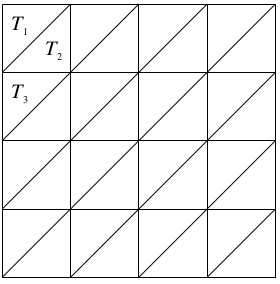
\includegraphics{../image/Fig.11.1.png}
%		\caption{单位正方形的规则三角剖分}
%	\end{figure}

\begin{figure}[ht]
	\centering
	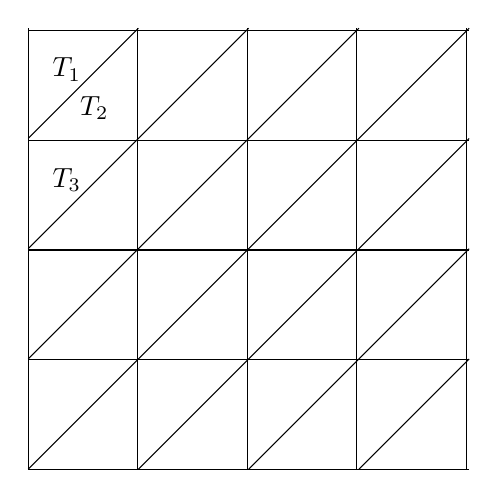
\begin{tikzpicture}[scale=0.7]
		\draw [step=56.56pt] (0,8) grid (8,0);
		
		\draw (0,6) -- (2,8);
		\draw (0,4) -- (4,8);
		\draw (0,2) -- (6,8);
		\draw (0,0) -- (8,8);
		\draw (2,0) -- (8,6);
		\draw (4,0) -- (8,4);
		\draw (6,0) -- (8,2); 
		
		\node at(0.7,7.25) {$T_1$};
		\node at(1.2,6.55) {$T_2$};
		\node at(0.7,5.25) {$T_3$};
	\end{tikzpicture}
	\caption{}
	\label{pf}
\end{figure}
	
	定义 $L_{\lambda,h}$ 为
	\begin{equation}
	L_{\lambda,h} := sup \{ \frac{|u-u_h^{\lambda}|_{H^1(\Omega)}}{\| div \sigma_{\lambda}(u) \|_{L^2(\Omega)}} : 0 \ne u \in H^2(\Omega) \cap H^1(\Omega) \}.
	\end{equation}
	\\ 
	则存在一个与 $h$ 无关的正常数 $C$ 使得\textsuperscript{\cite{brenner2008mathematical}}
	\begin{equation}
	\lim\limits_{\lambda \to \infty} \inf L_{\lambda,h} \ge C . \label{ab}
	\end{equation}
	式 $\eqref{ab}$ 意味着:无论 $h$ 取多小,只要 $\lambda$ 足够大,我们都能找到 $u \in H^2(\Omega) \cap H^1(\Omega)$ 使得相对误差$ |u-u_h|_{H^1(\Omega)} / \| div \sigma_{\lambda}(u) \|_{L^2(\Omega)} $ 以一个与 $h$ 无关的常数为下界。换句话说,有限元方法的性能将会随着 $\lambda$ 变大而变坏。
	\par
	\iffalse
	为证明式 $\eqref{ab}$,首先观察到
	$$
	\{ \nu \in V_h : div \nu = 0 \} = \{ 0 \}
	$$
	因此,映射 $\nu \to div \nu$ 是有限维空间 $V_h$ 到 $L^2(\Omega)$ 的一个一对一映射,并且存在一个正常数 $C_1(h)$ 使得
	$$
	\| \nu \|_{H^1(\Omega)} \le C_1(h) \| div \nu \|_{L^2(\Omega)} \quad \forall \nu \in V_h.
	$$
	令 $\psi$ 是 $\overline{\Omega}$ 上的无穷次可微函数,使得在 $\Omega$ 的边界上 $curl \psi = 0$ 且 $\| \epsilon(curl \psi) \|_{L^2(\Omega)} = 1$。令 $u := curl \psi$。则 $u \in H^2(\Omega) \cap H^1(\Omega)$,并有
	\begin{align}	
	div u = 0, \label{a2} \\
	\| \epsilon(u) \|_{L^2(\Omega)} = 1, \label{a3}\\
	\sigma_{\lambda}(u) = 2 \epsilon(u).  \label{a4}
	\end{align}
	根据 $\eqref{a2}$, $\eqref{a4}$ 和分步积分得
	\begin{align}
	- \int_{\Omega} div \epsilon(u) \cdot u dx = \int_{\Omega} \epsilon(u) : \epsilon(u) dx = 1. \label{a5}
	\end{align}
	根据 $\eqref{a4}$, $\eqref{a5}$ 推断
	$$
	\quad \quad \quad \quad \quad \quad \quad
	\lim\limits_{\lambda \to \infty} div \sigma_{\lambda}(u) = 2 div \epsilon(u) \ne 0. 
	$$
	由 (2.5.10) 得,
	$$
	a_{\lambda}(u-u_h^{\lambda}, u-u_h^{\lambda}) = \min\limits_{\nu \in V_h} a_{\lambda}(u-\nu,u-\nu) \le a_{\lambda}(u,u).
	$$
	由 $\eqref{a2}$ 和 $\eqref{a3}$,得到
	$$
	a_{\lambda}(u,u) = 2.
	$$
	因此,对于 $\lambda$ 足够大时有
	\begin{align} 
	a_{\lambda} (u-u_h^{\lambda}, u-u_h^{\lambda}) \le 2. \label{a6}
	\end{align}
	由 $\eqref{a2}$ 和 $\eqref{a6}$ 得
	\\
	$$
	\begin{matrix}
		\sqrt{\lambda} \| div u_h^{\lambda} \|_{L^2(\Omega)} = \sqrt{\lambda} \| div(u-u_h^{\lambda}) \|_{L^2(\Omega)} \\ 
		\quad \quad \quad \quad \quad \quad \quad
		\le \sqrt{a_{\lambda}(u-u_h^{\lambda}, u-u_h^{\lambda})} \\
		\le \sqrt{2}	
	\end{matrix}
	$$
	\\
	对足够大的 $\lambda$ 有
	$$
	\lim\limits_{\lambda \to \infty} \| div u_h^{\lambda} \|_{L^2(\Omega)} = 0.
	$$
	\\
	由式 $\eqref{ab}$ 有
	$$
	\lim\limits_{\lambda \to \infty} \| u_h^{\lambda} \|_{H^1(\Omega)} = 0.
	$$
	最后,得到 %(cf.exercise 11.x.16)
	$$ 
	\begin{matrix}
		\lim\limits_{\lambda \to \infty}\inf L_{\lambda,h} \ge \lim\limits_{\lambda \to \infty}\inf \frac{|u-u_h^{\lambda}|_{H^1(\Omega)}}{\| div \sigma_{\lambda}(u) \|_{L^2(\Omega)}} \\
		\quad \quad \quad \quad
		= \frac{|u|_{H^1(\Omega)}}{\| div \sigma(u) \|_{L^2(\Omega)}} > 0.
	\end{matrix}
	$$
	\fi

令 $\Omega = (0,1) \times (0,1).$ 考虑以下纯位移问题
\begin{equation}
\begin{aligned}
	-\mu \, \bigtriangleup u - (\mu + \lambda) \, grad \, (div \, u) &= f \quad \in \Omega, \\
	u &= 0 \quad \, on \, \, \partial \Omega ,
	\label{11.4.1}
\end{aligned}
\end{equation}
其中,$f \in L^2(\Omega), \, \Omega_1, \, \Omega_2$ 是 $\Omega$ 的两个子集,使得 $\Omega_1 \bigcup \Omega_2 = \Omega$ 并且 $\Omega_1 \bigcap \Omega_2 = \emptyset, \, (x,y) \in \Omega_1$ 时 $\lambda = \lambda_1, \, \mu = \mu_1, \, (x,y) \in \Omega_2$ 时 $\lambda = \lambda_2, \, \mu = \mu_2, \, \lambda_1 \ne \lambda_2, \, \mu_1 \ne \mu_2.$ 

它的变分形式为,求 $u \in H^1(\Omega)$ 使得 $u|_{\Gamma} = 0,$ 并且
\begin{equation}
	a^s(u,v) = \int_{\Omega} \, f \cdot v \, dxdy \quad \forall v \in H^1(\Omega),
\end{equation}
其中
\begin{equation}
	a^s(u, v) = \mu \, \int_{\Omega} \, grad \, u : grad \, v \, dxdy + (\mu +\lambda) \int_{\Omega} \, (div \, u) \, (div \, v) \, dxdy .
\end{equation}

令$\emph{T}^h$ 是$\Omega$ 三角划分的一个非退化族。定义
\begin{equation}
\begin{aligned}
	V_h^{\star} = \{v : v \in L^2(\Omega), \, v|_{T} \mbox{是线性的} \, \forall \emph{T} \in \emph{T}^h, \\
	 v \mbox{在单元边界的中点上是连续的并且} v = 0 \} .
\end{aligned}
\end{equation}
对 $v \in V_h^{\star},$ 定义
\begin{equation}
	(grad_h \, v) |_{\emph{T}} = grad \, (v|_{\emph{T}}), \quad
	(div_h \, v) |_{\emph{T}} = div \, (v|_{\emph{T}}), \quad
	\forall \emph{T} \in \emph{T}^h. 
\end{equation}

则问题的离散形式为,求 $u_h \in V_h^{\star}$ 使得
\begin{equation}
	a_h^{\star}(u_h, v) = \int_{\Omega} \, f \cdot v \, dxdy, \quad \forall v \in V_h^{\star},
\end{equation}
其中双线性形式 $a_h^{\star}(\cdot, \cdot)$ 在 $V_h^{\star} + H^1(\Omega)$ 上的定义为
\begin{equation}
\begin{aligned}
	a_h^{\star} (u, v) &= \mu \, \int_{\Omega} \, grad_h \, u : grad_h \, v \, dxdy \\ 
	&+ (\mu + \lambda) \, \int_{\Omega} \, (div_h \, u) \, (div_h \, v) \, dxdy.
\end{aligned}
\label{11.4.8}
\end{equation}

定义 $V_h^{\star} + H^1(\Omega)$ 上的非协调能量泛函
\begin{equation}
	|| v ||_h = a_h^{\star} (v,v)^{1/2}.
	\label{11.4.9}
\end{equation}
显然
\begin{equation}
	|| grad_h \, v ||_{L^2(\Omega)} \le \mu^{-1/2} || v ||_h.
	\label{11.4.10}
\end{equation}

定义
\begin{equation}
	(\Pi_h u)(m_e) = \frac{1}{|e|} \int_e \, u \, ds,
	\label{11.4.12}
\end{equation}
其中$m_e$ 为边缘 $e$ 的中点。则有
\begin{equation}
	div(\Pi_h u)|_{\emph{T}} = \frac{1}{|\emph{T}|} \int_{\emph{T}} \, div \, u \, dxdy \quad \forall \emph{T} \in \emph{T}^h,
	\label{11.4.13}
\end{equation}
并且存在独立于 $h$ 的正常数 $C$ 使得
\begin{equation}
	|| u - \Pi_h u ||_{L^2(\Omega)} + h ||grad_h \, (u-\Pi_h u) ||_{L^2(\Omega)} \le C h^2 |u|_H^2(\Omega).
	\label{11.4.14}
\end{equation}
参考文献得
\begin{equation}
	||u||_{H^2(\Omega)} + \lambda ||div \, u||_{H^1(\Omega)} 
	\le C ||f||_{L^2(\Omega)} ,
	\label{11.4.4}
\end{equation}

\begin{equation}
	|| u - u_h ||_h \le \inf_{v \in V_h} \, ||u-v||_h + \sup_{v \in V_h \backslash \{0\}} \frac{|a_h^s(u,v) - \int_{\Omega} \, f \cdot v 
	\, dxdy|}{||v||_h} ,
	\label{11.4.17}
\end{equation}

\begin{equation}
\begin{aligned}
	\arrowvert \int_{\Omega} \, grad_h \, u : grad_h \, v \, dxdy + \int_{\Omega} \bigtriangleup u \cdot v \, dxdy \arrowvert \\
	\le C \, h \, |u|_{H^2(\Omega)} ||grad_h \, v||_{L^2(\Omega)},
\end{aligned}
\label{11.4.18}
\end{equation}

\begin{equation}
\begin{aligned}
	|\int_{\Omega} \, div_h \, u \, div_h \, v \, dxdy + \int_{\Omega} \, grad \, (div \, u) \cdot v \, dxdy| \\
	\le C \, h \, |div \, u|_{H^1(\Omega)} ||grad_h \, v||_{L^2(\Omega)}.
\end{aligned}
\label{11.4.19}
\end{equation}

设
\begin{equation}
\begin{aligned}
	a^s(u, v) |_{\Omega_1} &= \mu \, \int_{\Omega_1} \, grad \, u : grad \, v \, dxdy \\
	&+ (\mu +\lambda) \int_{\Omega_1} \, (div \, u) \, (div \, v) \, dxdy .
\end{aligned}
\end{equation}
由公式 $\eqref{11.4.1}, \eqref{11.4.8}, \eqref{11.4.18}, \eqref{11.4.19}, \eqref{11.4.4}$ 和 $\eqref{11.4.10}$ 得

\begin{equation}
\begin{aligned}
	&|a_h^s(u,v) - \int_{\Omega} \, f \cdot v \, dxdy| \\
	&= |(a_h^s(u,v)|_{\Omega_1} - \int_{\Omega} \, f \cdot v \, dxdy) \\
	&+ (a_h^s(u,v)|_{\Omega_2} - \int_{\Omega} \, f \cdot v \, dxdy)|\\
	&\le C \, h \, ||grad_h \, v||_{L^2(\Omega_1)} (\mu_1 |u|_{H^2(\Omega_1)} + (\mu_1+\lambda_1) |div \, u|_{H^1(\Omega_1)}) \\
	&+ C \, h \, ||grad_h \, v||_{L^2(\Omega_2)} (\mu_2 |u|_{H^2(\Omega_2)} + (\mu_2+\lambda_2) |div \, u|_{H^1(\Omega_2)}) \\
	&\le C \, h \, ||v||_h ||f||_{L^2(\Omega)}. 
\end{aligned}
\label{11.4.20}
\end{equation}
参考文献得到,存在 $u_1 \in H^2(\Omega) \cup H^1(\Omega),$ 使得
\begin{equation}
	div \, u_1 = div \, u ,
	\label{11.4.21}
\end{equation}

\begin{equation}
	||u_1||_{H^2(\Omega)} \le C \, ||div \, u||_{H^1(\Omega)} ,
	\label{11.4.22}
\end{equation}

\begin{equation}
	||u_1||_{H^2(\Omega)} \le \frac{C}{1+\lambda} \, ||f||_{L^2(\Omega)} ,
	\label{11.4.23}
\end{equation}

\begin{equation}
	div_h \, \Pi_h \, u_1 = div_h \, \Pi_h \, u.
	\label{11.4.24}
\end{equation}

由公式 $\eqref{11.4.4}, \eqref{11.4.14}, \eqref{11.4.21}, \eqref{11.4.23}$ 和 $\eqref{11.4.24}$ 得
\begin{equation}
\begin{aligned}
	&\inf_{v \in V_h} ||u - v||_h \\
	&\le ||u - \Pi_h u||_h \\
	&= (\mu_1 ||grad_h \, (u-\Pi_h u)||_{L^2(\Omega_1)}^2 + (\mu_1+\lambda_1) ||div_h \, (u-\Pi_h u)||^2_{L^2(\Omega_1)})^{1/2} \\
	&+ (\mu_2 ||grad_h \, (u-\Pi_h u)||_{L^2(\Omega_2)}^2 + (\mu_2+\lambda_2) ||div_h \, (u-\Pi_h u)||^2_{L^2(\Omega_2)})^{1/2} \\
	&= (\mu_1 ||grad_h \, (u-\Pi_h u)||_{L^2(\Omega_1)}^2 + (\mu_1+\lambda_1) ||div_h \, (u_1-\Pi_h u_1)||^2_{L^2(\Omega_1)})^{1/2} \\
	&+ (\mu_2 ||grad_h \, (u-\Pi_h u)||_{L^2(\Omega_2)}^2 + (\mu_2+\lambda_2) ||div_h \, (u_1-\Pi_h u_1)||^2_{L^2(\Omega_2)})^{1/2} \\
	&\le C \, h \, ||f||_{L^2(\Omega)}.
\end{aligned}
\label{11.4.25}
\end{equation}

由公式 $\eqref{11.4.17}, \eqref{11.4.20}, \eqref{11.4.25}$ 得
\begin{equation}
	||u-u_h||_h \le C \, h \, ||f||_{L^2(\Omega)}.
\end{equation}

\clearpage
%\newpage

\section{算例}

\subsection{弹性问题}

\subsubsection{算例一}

考察以下边值问题
$$
\begin{matrix}
	-div \, \sigma(u) = f \quad \in \Omega , \\
	u |_{\partial \Omega} = 0 .
	%(\sigma(u) \nu) |_{\Gamma2} = t
\end{matrix}
$$ 
其中$ u = (u_1,u_2)^t $ 为求解向量,$ f = (f_1,f_2)^t $为右端向量,$ \Omega = [0,1] \times [0,1], $
$$
\begin{matrix}
	u_1 = (x - 1)(y - 1) y sin(x) ,
	\\
	u_2 = (x - 1)(y - 1) x sin(y) .
\end{matrix}
$$
通过数值实验得到,
\begin{enumerate}
\item 当Lam$\acute{e}$ 常数 $\mu =1, \, \lambda = 1$ 时的误差及误差阶如下表

\begin{table}[h]
	\centering
	\caption{}
	\scalebox{0.8}{
		\begin{tabular}{|c|c|c|c|c|} \hline
			h &1.0 &0.5 &0.25 &0.125  \\ \hline
			$|u-u_h|_{H^1(\Omega)}$ &4.102804E-1 &1.424371E-1 &8.382384E-2 &4.737414-2  \\ \hline
			H1误差阶 &1.526284 &0.764893 &0.823260 &0.905945 \\ \hline
			$|u-u_h|_{L^2(\Omega)}$ &4.102632E-1 &7.121859E-2 &2.095596E-2 &5.921768E-3  \\ \hline
			L2误差阶 &2.526284 &1.764893 &1.823260 &1.905945 \\ \hline	
	\end{tabular}}
\end{table}

\item 当Lam$\acute{e}$ 常数 $\mu =1, \, \lambda = 1E4$ 时的误差及误差阶如下表

\begin{table}[h]
	\centering
	\caption{}
	\scalebox{0.8}{
		\begin{tabular}{|c|c|c|c|c|} \hline
			h &1.0 &0.5 &0.25 &0.125  \\ \hline
			$|u-u_h|_{H^1(\Omega)}$ &3.954836E-1 &1.369558E-1 &8.048234E-2 &4.543017E-2   \\ \hline
			H1误差阶 &1.529907 &0.7669663 &0.8250215 &0.9072268 \\ \hline
			$|u-u_h|_{L^2(\Omega)}$ &3.945746E-1 &6.847791E-2 &2.012058E-2 &5.678771E-3  \\ \hline
			L2误差阶 &2.529607 &1.766966 &1.825021 &1.907226 \\ \hline	
	\end{tabular}}
\end{table}

\item 当Lam$\acute{e}$ 常数 $\mu =1, \, \lambda = 1E8$ 时的误差及误差阶如下表

\begin{table}[h]
	\centering
	\caption{}
	\scalebox{0.8}{
		\begin{tabular}{|c|c|c|c|c|} \hline
			\diagbox{$\lambda$}{h} &1.0 &0.5 &0.25 &0.125  \\ \hline
			$|u-u_h|_{H^1(\Omega)}$ &4.102771E-1 &1.424359E-1 &8.382310E-2 &4.737371E-2  \\ \hline
			H1误差阶 &1.526285 &0.7648937 &0.823261 &0.9059459 \\ \hline
			$|u-u_h|_{L^2(\Omega)}$ &4.104650E-1 &7.121799E-2 &2.095577E-2 &5.921714E-3  \\ \hline
			L2误差阶 &2.526285 &1.764893 &1.823261 &1.905945 \\ \hline	
	\end{tabular}}
\end{table}

\end{enumerate}
\newpage
数值解和精确解图像如下

\begin{figure}[ht]
	\centering
	\caption{}
	\subfigure[数值解图像]{
		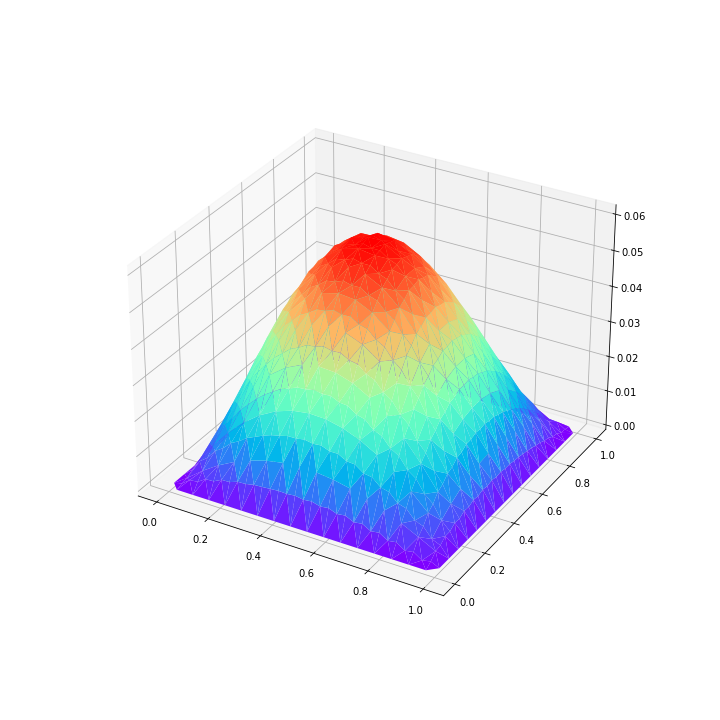
\includegraphics[height=5.5cm,width=5.5cm]{../image/elaticity_uh_u/PDE1/uh_lam=1.png}
		\label{elsticity_uh_1}}	
	\subfigure[精确解图像]{
		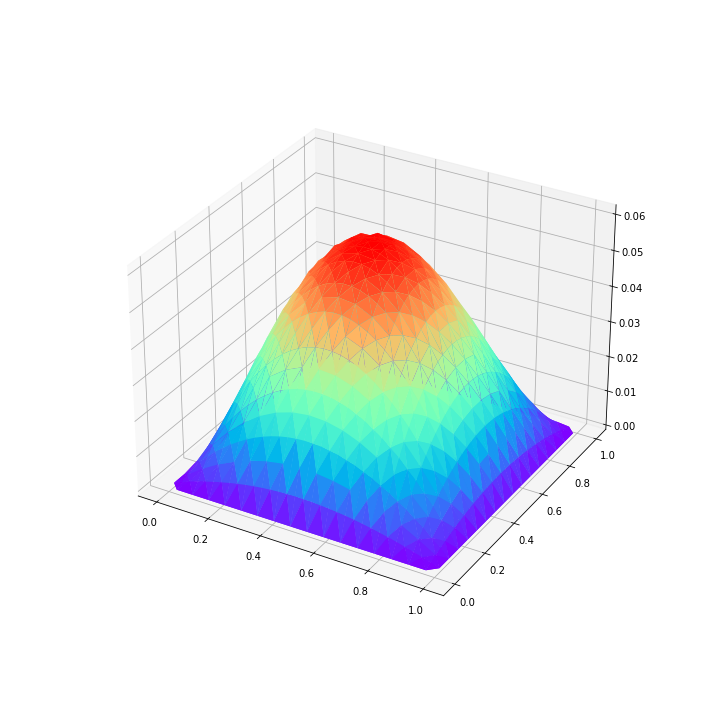
\includegraphics[height=5.5cm,width=5.5cm]{../image/elaticity_uh_u/PDE1/u_lam=1.png}
		\label{elsticity_u_1}}
\end{figure}
\newpage
\subsubsection{算例二}

考察以下边值问题
$$
\begin{matrix}
	-div \, \sigma(u) = f \quad \in \Omega , \\
	u |_{\partial \Omega} = 0 .
	%(\sigma(u) \nu) |_{\Gamma2} = t
\end{matrix}
$$ 
其中$ u = (u_1,u_2)^t $ 为求解向量,$ f = (f_1,f_2)^t $为右端向量,$ \Omega = [0,1] \times [0,1] ,$
$$
\begin{matrix}
	u_1 = x^2 sin(x-1) y^2 sin(y-1) ,
	\\
	u_2 = x^2 sin(x-1) y^2 sin(y-1) .
\end{matrix}
$$
通过数值实验得到,

\begin{enumerate}
	\item 当Lam$\acute{e}$ 常数 $\mu =1, \, \lambda = 1$ 时的误差及误差阶如下表
	
	\begin{table}[h]
		\centering
		\caption{}
		\scalebox{0.8}{
			\begin{tabular}{|c|c|c|c|c|} \hline
				h &1.0 &0.5 &0.25 &0.125  \\ \hline
				$|u-u_h|_{H^1(\Omega)}$ &1.381670E-1 &1.038442E-1 &4.190134E-2 &2.135923E-2  \\ \hline
				H1误差阶 &0.4119931 &1.309352 &0.972136 &0.9399994 \\ \hline
				$|u-u_h|_{L^2(\Omega)}$ &1.435610E-1 &5.192211E-2 &1.047533E-2 &2.669904E-3  \\ \hline
				L2误差阶 &1.411993 &2.309352 &1.972136 &1.939999 \\ \hline	
		\end{tabular}}
	\end{table}
	
	\item 当Lam$\acute{e}$ 常数 $\mu =1, \, \lambda = 1E4$ 时的误差及误差阶如下表
	
	\begin{table}[h]
		\centering
		\caption{}
		\scalebox{0.8}{
			\begin{tabular}{|c|c|c|c|c|} \hline
				h &1.0 &0.5 &0.25 &0.125  \\ \hline
				$|u-u_h|_{H^1(\Omega)}$ &1.328102E-1 &1.001068E-1 &4.029172E-2 &2.049834E-2   \\ \hline
				H1误差阶 &0.4078262 &1.312984 &0.9749761 &0.9414672 \\ \hline
				$|u-u_h|_{L^2(\Omega)}$ &1.647602E-1 &5.005340E-2 &1.007293E-2 &2.562293E-3  \\ \hline
				L2误差阶 &1.407826 & 2.312984 &1.974976 &1.941467 \\ \hline	
		\end{tabular}}
	\end{table}
	
	\item 当Lam$\acute{e}$ 常数 $\mu =1, \, \lambda = 1E8$ 时的误差及误差阶如下表
\newpage	
	\begin{table}[h]
		\centering
		\caption{}
		\scalebox{0.8}{
			\begin{tabular}{|c|c|c|c|c|} \hline
				\diagbox{$\lambda$}{h} &1.0 &0.5 &0.25 &0.125  \\ \hline
				$|u-u_h|_{H^1(\Omega)}$ &1.381659E-1 &1.038433E-1 &4.190099E-2 &2.135904E-2  \\ \hline
				H1误差阶 &0.4119922 &1.309353 &0.9721372 &0.9399997 \\ \hline
				$|u-u_h|_{L^2(\Omega)}$ &1.473169E-1 &5.192169E-2 &1.047524E-2 &2.669880E-3  \\ \hline
				L2误差阶 &1.411992 &2.309353 &1.972137 &1.939999 \\ \hline	
		\end{tabular}}
	\end{table}
	
\end{enumerate}

数值解和精确解图像如下

\begin{figure}[ht]
	\centering
	\caption{}
	\subfigure[数值解图像]{
		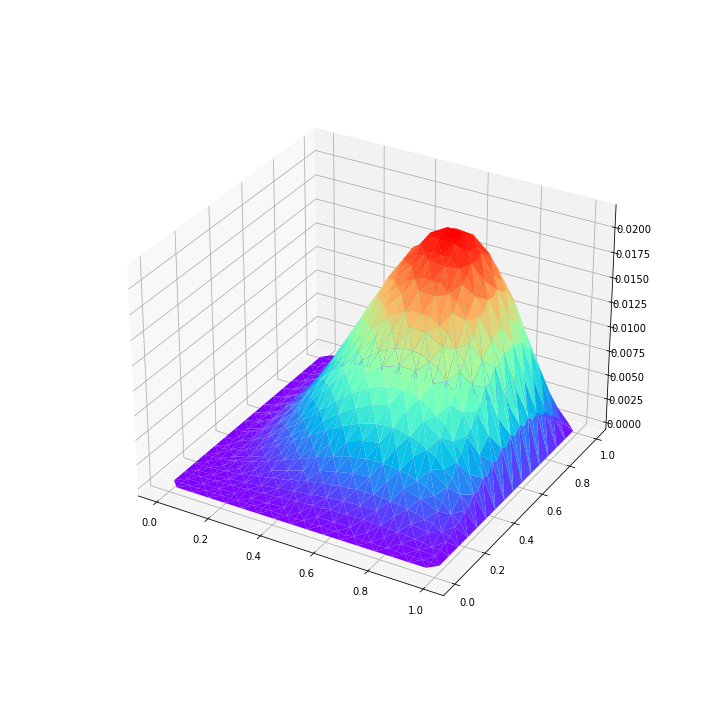
\includegraphics[height=5.5cm,width=5.5cm]{../image/elaticity_uh_u/PDE2/uh_lam=1.png}
		\label{elsticity_uh_2}}	
	\subfigure[精确解图像]{
		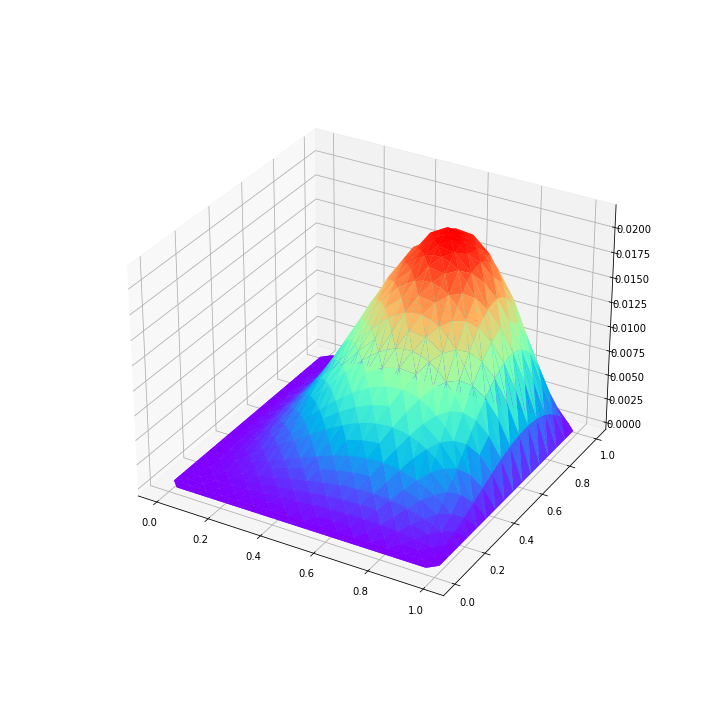
\includegraphics[height=5.5cm,width=5.5cm]{../image/elaticity_uh_u/PDE2/u_lam=1.png}
		\label{elsticity_u_2}}
\end{figure}

\iffalse
\newpage

\subsubsection{算例三}

考察以下边值问题
$$
\begin{matrix}
	-div \, \sigma(u) = f \quad \in \Omega  \\
	u |_{\partial \Omega} = 0 .
	%(\sigma(u) \nu) |_{\Gamma2} = t
\end{matrix}
$$ 
\par
其中$ u = (u_1,u_2)^t $ 为求解向量,$ f = (f_1,f_2)^t $为右端向量,$ \Omega = [0,1] \times [0,1] $
$$
\begin{matrix}
	u_1 = -(x-1) (e^x-1) (y-1) (e^y-1) ,
	\\
	u_2 = -(x-1) (e^x-1) (y-1) (e^y-1) .
\end{matrix}
$$

通过数值实验得到,当Lam$\acute{e}$ 常数 $\mu =1$, $\lambda = 1, 1E4, 1E8$ 时的误差及误差阶如下表

\begin{table}[ht]
	\centering
	\caption{$|u-u_h|_{H^1(\Omega)}$}
	\scalebox{0.8}{
		\begin{tabular}{|c|c|c|c|c|c|c|} \hline
			\diagbox{$\lambda$}{h} &1.0 &0.5 &0.25 &0.125 &0.0625 &误差阶 \\ \hline
			1 &8.170963E-1 &3.487612E-1 &1.669124E-1 &8.921846E-2 &4.718501E-2 &0.9561194 \\ \hline
			1E4 &7.867187E-1 &3.356780E-1 &1.601207E-1 &8.542417E-2 &4.513468E-2 &0.9590752  \\ \hline
			1E8 &8.170896E-1 &3.487583E-1 &1.669109E-1 &8.921763E-2 &4.718456E-2 &0.9561200 \\ \hline
	\end{tabular}}
\end{table}

数值解和精确解图像如下

\begin{figure}[h]
	\centering
	\caption{}
	\subfigure[数值解图像]{
		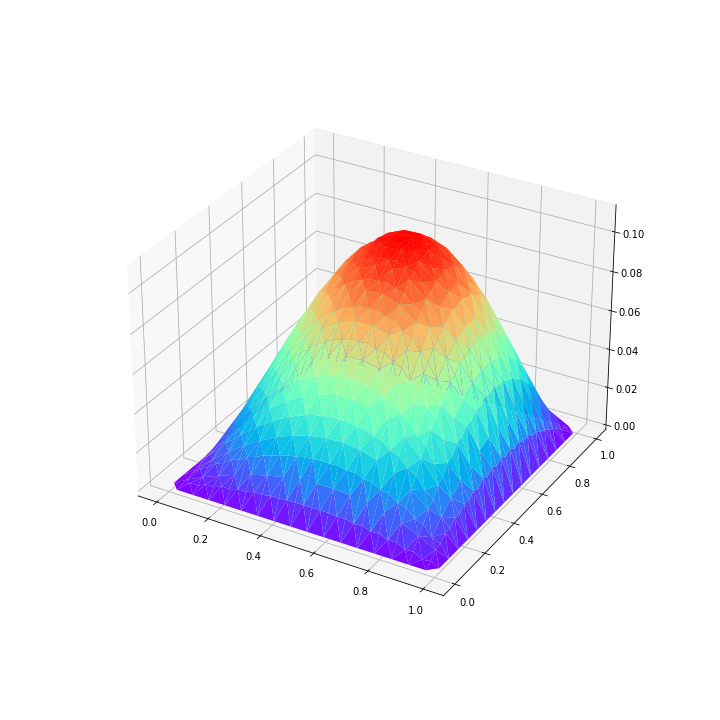
\includegraphics[height=5.5cm,width=5.5cm]{../image/elaticity_uh_u/PDE3/uh_lam=1.png}
		\label{elsticity_uh_3}}	
	\subfigure[精确解图像]{
		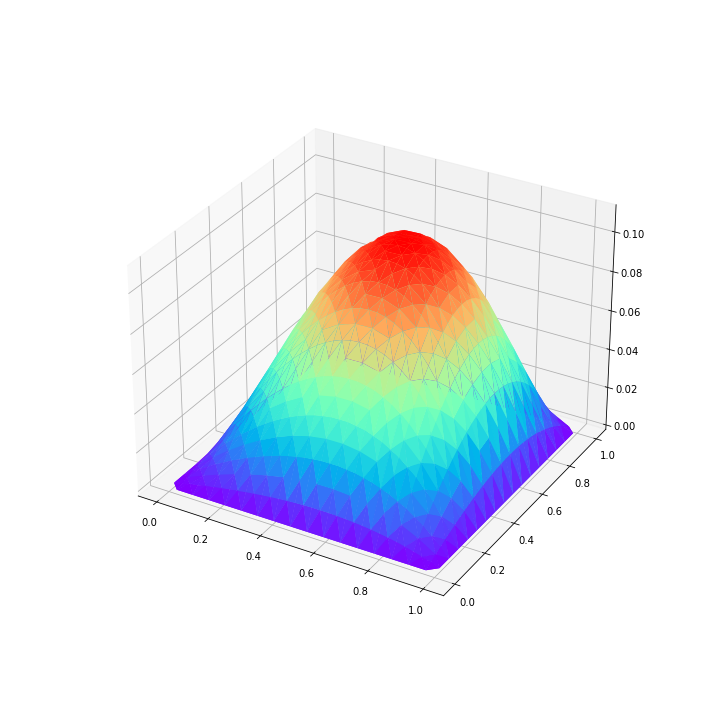
\includegraphics[height=5.5cm,width=5.5cm]{../image/elaticity_uh_u/PDE3/u_lam=1.png}
		\label{elsticity_u_3}}
\end{figure}
\fi
\newpage

\subsection{带间断系数的弹性问题}

\subsubsection{算例一}

考察以下边值问题
$$
\begin{matrix}
	-div \, \sigma(u) = f \quad \in \Omega , \\
	u |_{\Gamma} = 0 .
	%(\sigma(u) \nu) |_{\Gamma2} = t
\end{matrix}
$$ 
\par
其中$ u = (u_1,u_2)^t $ 为求解向量,$ f = (f_1,f_2)^t $为右端向量,
$ 
\Omega = [0,1] \times [0,1] , \quad 
\Omega_1 = [0,0.5] \times [0,0.5] , \quad
\Omega_2 = [0.5,1] \times [0,0.5], \quad
\Omega_3 = [0,0.5] \times [0.5,1], \\
\Omega_4 = [0.5,1] \times [0.5,1].
$ 
\par
当$(x,y) \in \Omega_1$时,$\mu = \lambda = \lambda_1,$
$$
\begin{matrix}
	u_1 = x (x-0.5) (x-1) y (y-0.5) (y-1) \, / \, \lambda_1 ,
	\\
	u_2 = x (x-0.5) (x-1) y (y-0.5) (y-1) \, / \, \lambda_1 .
\end{matrix}
$$

当$(x,y) \in \Omega_2$时, $\mu = \lambda = \lambda_2,$

$$
\begin{matrix}
	u_1 = x (x-0.5) (x-1) y (y-0.5) (y-1) \, / \, \lambda_2 ,
	\\
	u_2 = x (x-0.5) (x-1) y (y-0.5) (y-1) \, / \, \lambda_2 .
\end{matrix}
$$

当$(x,y) \in \Omega_3$时,$\mu = \lambda = \lambda_3,$ 
$$
\begin{matrix}
	u_1 = x (x-0.5) (x-1) y (y-0.5) (y-1) \, / \, \lambda_3 ,
	\\
	u_2 = x (x-0.5) (x-1) y (y-0.5) (y-1) \, / \, \lambda_3 .
\end{matrix}
$$

当$(x,y) \in \Omega_4$时, $\mu = \lambda = \lambda_4,$

$$
\begin{matrix}
	u_1 = x (x-0.5) (x-1) y (y-0.5) (y-1) \, / \, \lambda_4 ,
	\\
	u_2 = x (x-0.5) (x-1) y (y-0.5) (y-1) \, / \, \lambda_4 .
\end{matrix}
$$
令 $\lambda = [\lambda_1, \lambda_2, \lambda_3, \lambda_4]$,$\mu = [\mu_1, \mu_2, \mu_3, \mu_4].$ 

\clearpage

\begin{enumerate} 
	
\item 当Lam$\acute{e}$ 常数 $\lambda = \mu= [1,2,3,4]$ 时误差如下

\begin{table}[h]
	\centering
	\caption{}
	\scalebox{0.8}{
		\begin{tabular}{|c|c|c|c|c|} \hline
			h &0.5 &0.25 &0.125 &0.0625 \\ \hline
			$|u-u_h|_{H^1(\Omega)}$ &1.599642E-2 &7.130159E-3 &3.516517E-3 &1.900384E-3  \\ \hline
			H1误差阶 &1.165743 &1.019786 &0.8878559 &0.9186291 \\ \hline
			$|u-u_h|_{L^2(\Omega)}$ &3.999106E-3 &8.912698E-4 &2.197823E-4 &5.938701E-5  \\ \hline
			L2误差阶 &2.165743 &2.019786 &1.887855 &1.918629 \\ \hline	
	\end{tabular}}
\end{table}

\begin{figure}[h]
	\centering
	\caption{}
	\subfigure[数值解图像]{
		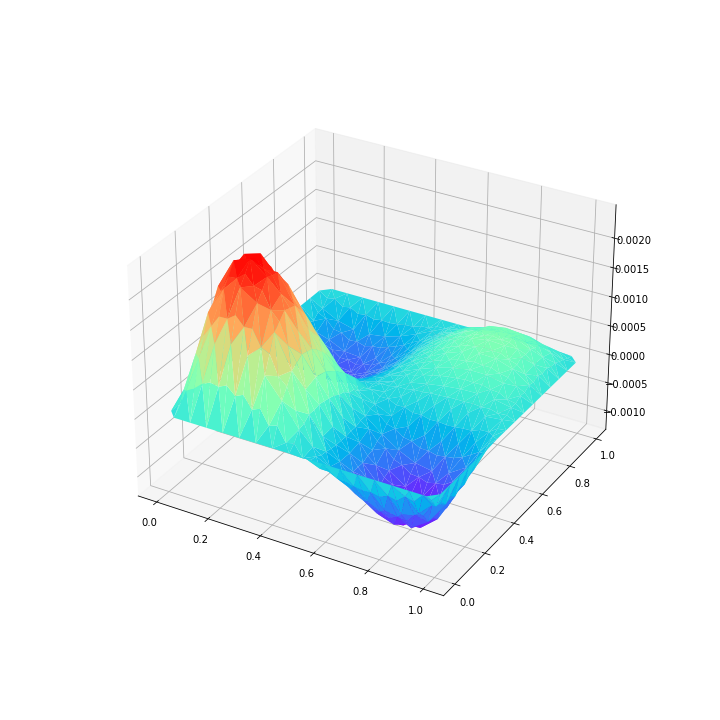
\includegraphics[height=5.7cm,width=5.7cm]{../image/interface_uh_u/uh_lam=[1. 2. 3. 4.].png}
		\label{interface_uh_0}}	
	\subfigure[精确解图像]{
		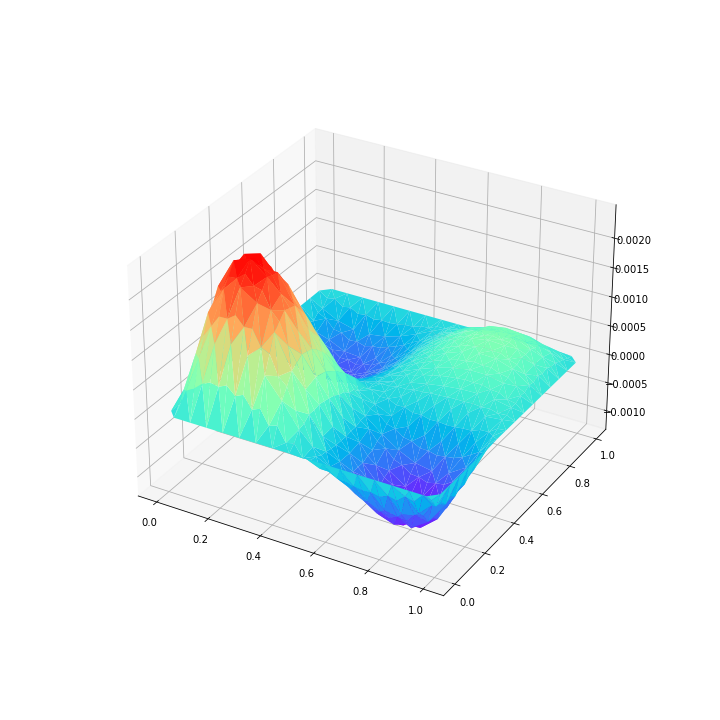
\includegraphics[height=5.7cm,width=5.7cm]{../image/interface_uh_u/uh_lam=[1. 2. 3. 4.].png}
		\label{interface_u_0}}
\end{figure}

\newpage

\item 当Lam$\acute{e}$ 常数 $\lambda = \mu= [1E4,2E4,3E4,4E4]$ 时误差如下

\begin{table}[h]
	\centering
	\caption{}
	\scalebox{0.8}{
		\begin{tabular}{|c|c|c|c|c|} \hline
			h &0.5 &0.25 &0.125 &0.0625 \\ \hline
			$|u-u_h|_{H^1(\Omega)}$ &1.599735E-2 &7.130099E-3 &3.516522E-3 &1.900428E-3  \\ \hline
			H1误差阶 &1.165839 &1.019772 &0.8878243 &0.918610 \\ \hline
			$|u-u_h|_{L^2(\Omega)}$ &3.999338E-3 &8.912623E-4 &2.197826E-4 &5.938839E-5  \\ \hline
			L2误差阶 &2.165839 &2.019772 &1.887824 &1.91861 \\ \hline	
	\end{tabular}}
\end{table}

\begin{figure}[h]
	\centering
	\caption{}
	\subfigure[数值解图像]{
		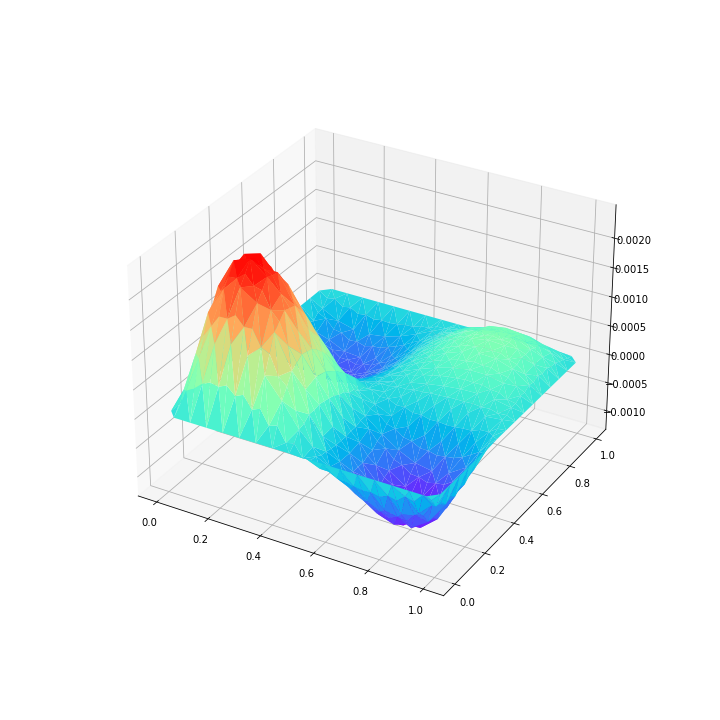
\includegraphics[height=5.7cm,width=5.7cm]{../image/interface_uh_u/uh_lam=[1. 2. 3. 4.].png}
		\label{interface_uh_4}}	
	\subfigure[精确解图像]{
		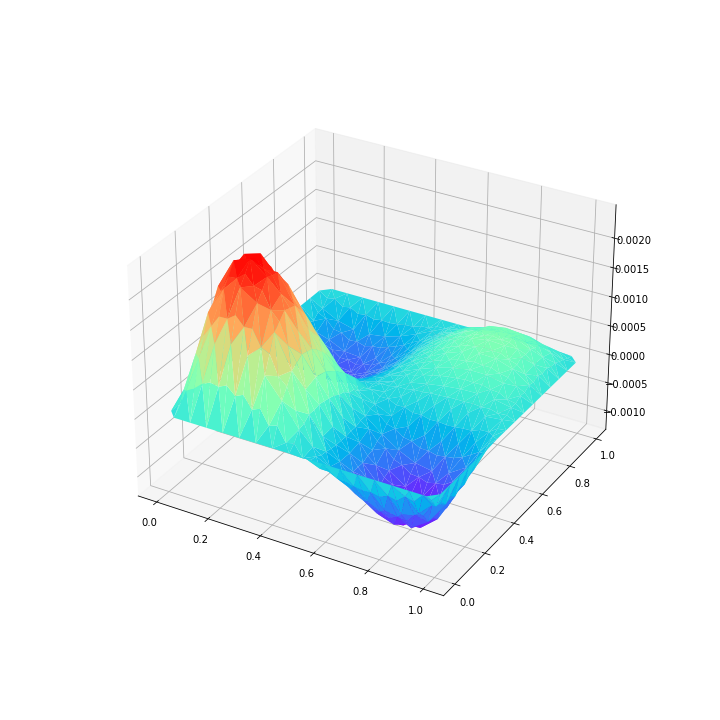
\includegraphics[height=5.7cm,width=5.7cm]{../image/interface_uh_u/uh_lam=[1. 2. 3. 4.].png}
		\label{interface_u_4}}
\end{figure}

\newpage

\item 当Lam$\acute{e}$ 常数 $\lambda = \mu= [1E8,2E8,3E8,4E8]$ 时误差如下

\begin{table}[h]
	\centering
	\caption{}
	\scalebox{0.8}{
		\begin{tabular}{|c|c|c|c|c|} \hline
			h &0.5 &0.25 &0.125 &0.0625 \\ \hline
			$|u-u_h|_{H^1(\Omega)}$ &3.015333E-3 &1.139928E-3 &6.718610E-4 &3.793589E-4  \\ \hline
			H1误差阶 &1.403373 &0.7627090 &0.8245995 &0.9054011 \\ \hline
			$|u-u_h|_{L^2(\Omega)}$ &7.538332E-4 &1.424911E-5 &4.199131E-5 &1.185496E-5  \\ \hline
			L2误差阶 &2.403373 &1.7627090 &1.824599 &1.905401 \\ \hline	
	\end{tabular}}
\end{table}

\begin{figure}[h]
	\centering
	\caption{}
	\subfigure[数值解图像]{
		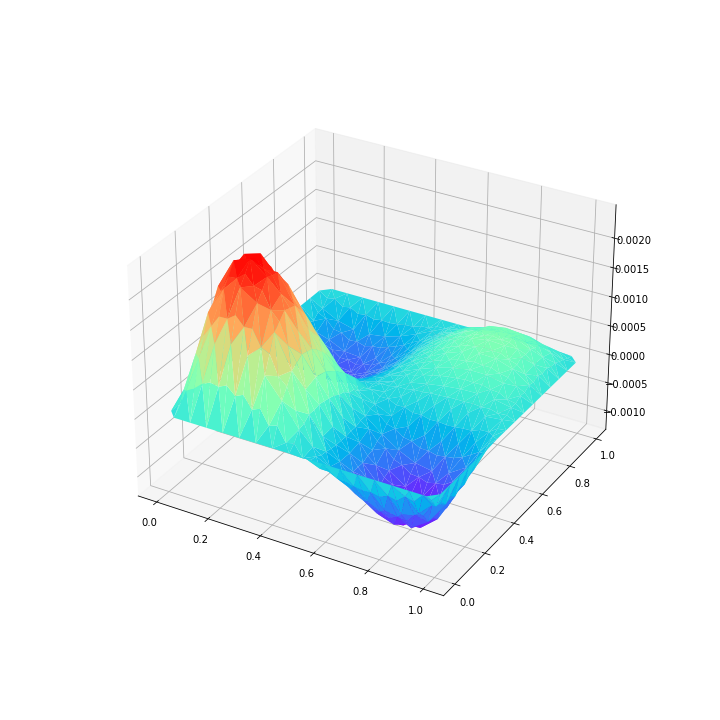
\includegraphics[height=5.7cm,width=5.7cm]{../image/interface_uh_u/uh_lam=[1. 2. 3. 4.].png}
		\label{interface_uh_8}}	
	\subfigure[精确解图像]{
		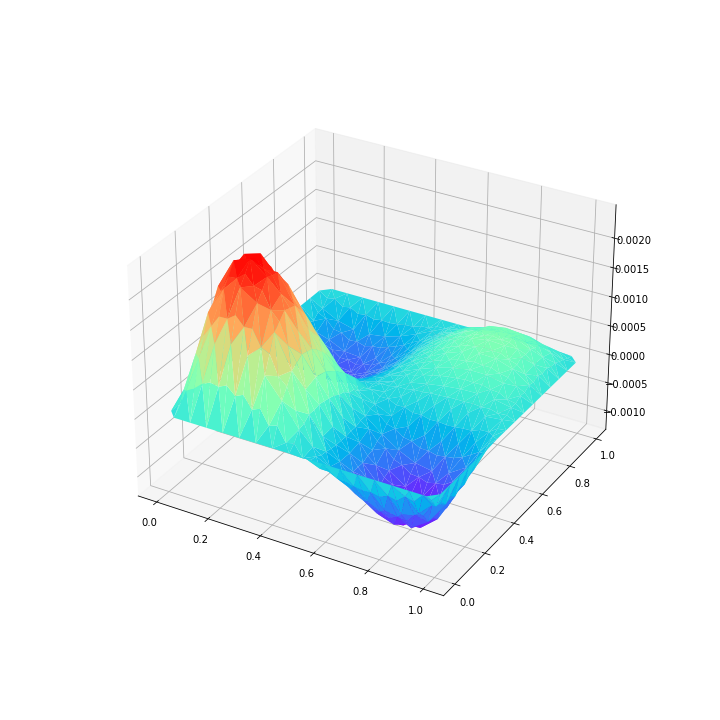
\includegraphics[height=5.7cm,width=5.7cm]{../image/interface_uh_u/uh_lam=[1. 2. 3. 4.].png}
		\label{interface_u_8}}
\end{figure}

\end{enumerate}

\newpage

\subsubsection{算例二}

考察以下边值问题
$$
\begin{matrix}
	-div \, \sigma(u) = f \quad \in \Omega , \\
	u |_{\Gamma} = 0 .
	%(\sigma(u) \nu) |_{\Gamma2} = t
\end{matrix}
$$ 
\par
其中$ u = (u_1,u_2)^t $ 为求解向量,$ f = (f_1,f_2)^t $为右端向量,
$ 
\Omega = [0,1] \times [0,1] , \quad 
\Omega_1 = [0,0.5] \times [0,0.5] , \quad
\Omega_2 = [0.5,1] \times [0,0.5], \quad
\Omega_3 = [0,0.5] \times [0.5,1], \quad
\Omega_4 = [0.5,1] \times [0.5,1].
$ 
\par
当$(x,y) \in \Omega_1$时,$\mu = \lambda = \lambda_1,$
$$
\begin{matrix}
	u_1 = \sin(\pi x) \, \cos(\pi x) \, \sin(\pi y) \, \cos(\pi y) \, / \, \lambda_1 ,
	\\
	u_2 = \sin(\pi x) \, \cos(\pi x) \, \sin(\pi y) \, \cos(\pi y) \, / \, \lambda_1 .
\end{matrix}
$$

当$(x,y) \in \Omega_2$时, $\mu = \lambda = \lambda_2,$

$$
\begin{matrix}
	u_1 = \sin(\pi x) \, \cos(\pi x) \, \sin(\pi y) \, \cos(\pi y) \, / \, \lambda_2 ,
	\\
	u_2 = \sin(\pi x) \, \cos(\pi x) \, \sin(\pi y) \, \cos(\pi y) \, / \, \lambda_2 .
\end{matrix}
$$

当$(x,y) \in \Omega_3$时,$\mu = \lambda = \lambda_3,$ 
$$
\begin{matrix}
	u_1 = \sin(\pi x) \, \cos(\pi x) \, \sin(\pi y) \, \cos(\pi y) \, / \, \lambda_3 ,
	\\
	u_2 = \sin(\pi x) \, \cos(\pi x) \, \sin(\pi y) \, \cos(\pi y) \, / \, \lambda_3 .
\end{matrix}
$$

当$(x,y) \in \Omega_4$时, $\mu = \lambda = \lambda_4,$

$$
\begin{matrix}
	u_1 = \sin(\pi x) \, \cos(\pi x) \, \sin(\pi y) \, \cos(\pi y) \, / \, \lambda_4 ,
	\\
	u_2 = \sin(\pi x) \, \cos(\pi x) \, \sin(\pi y) \, \cos(\pi y) \, / \, \lambda_4 .
\end{matrix}
$$
令 $\lambda = [\lambda_1, \lambda_2, \lambda_3, \lambda_4]$,$\mu = [\mu_1, \mu_2, \mu_3, \mu_4].$ 

\clearpage

\begin{enumerate} 
	
	\item 当Lam$\acute{e}$ 常数 $\lambda = \mu= [4,3,2,1]$ 时误差如下
	
	\begin{table}[h]
		\centering
		\caption{$|u-u_h|_{H^1(\Omega)}$}
		\scalebox{0.8}{
			\begin{tabular}{|c|c|c|c|c|} \hline
				h &0.5 &0.25 &0.125 &0.0625 \\ \hline
				$|u-u_h|_{H^1(\Omega)}$ &1.462698 &6.166073E-1 &4.261624E-1 &2.415138E-1 \\ \hline
				H1误差阶 &1.246208 &0.532948 &0.819297 &0.939899 \\ \hline 
				$|u-u_h|_{L^2(\Omega)}$ &7.313491E-1 &1.541518E-1 &5.327030E-2 &1.509461E-2  \\ \hline
				L2误差阶 &2.246208 &1.532948 &1.819297 &1.939899 \\ \hline
		\end{tabular}}
	\end{table}
	
	\begin{figure}[h]
		\centering
		\caption{}
		\subfigure[数值解图像]{
			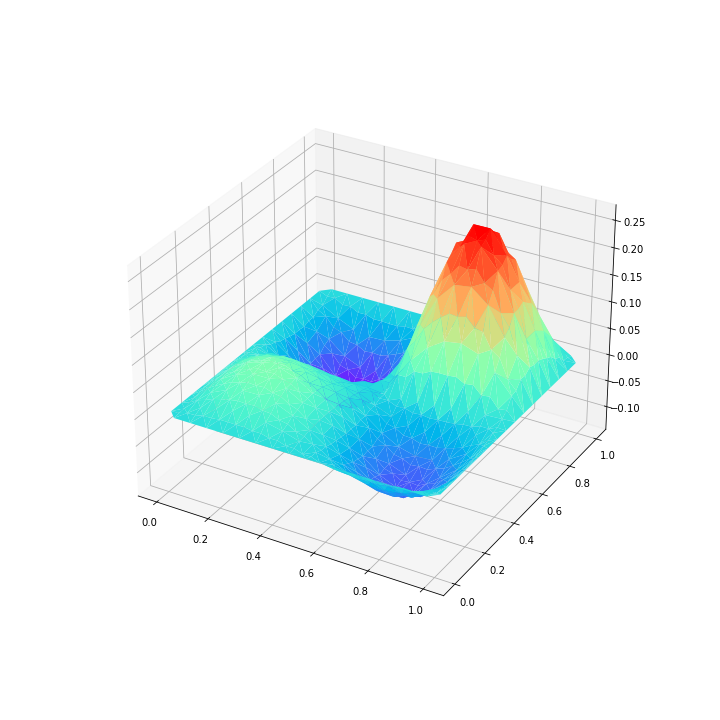
\includegraphics[height=5.7cm,width=5.7cm]{../image/interface_uh_u/interface2/uh_lam=[4. 3. 2. 1.].png}
			\label{interface2_uh_0}}	
		\subfigure[精确解图像]{
			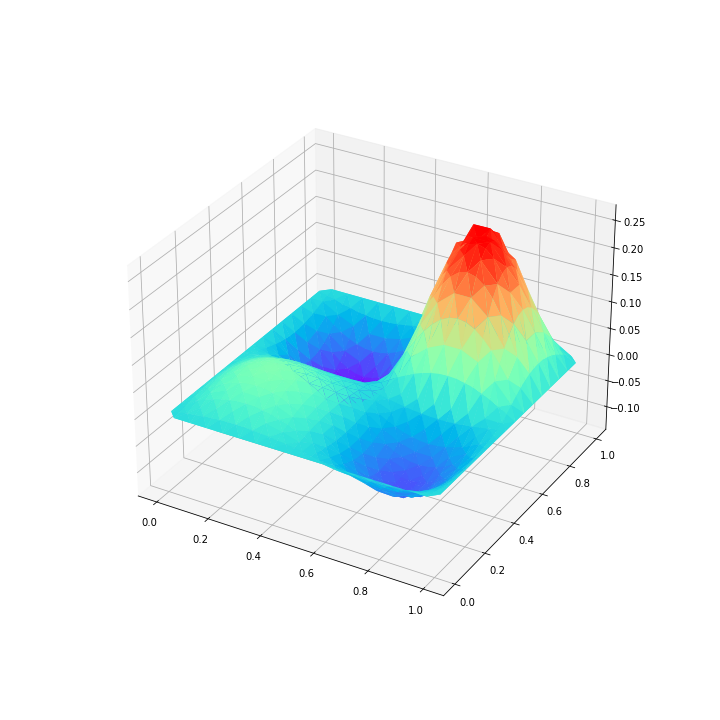
\includegraphics[height=5.7cm,width=5.7cm]{../image/interface_uh_u/interface2/u_lam=[4. 3. 2. 1.].png}
			\label{interface2_u_0}}
	\end{figure}
	
	\newpage
	
	\item 当Lam$\acute{e}$ 常数 $\lambda = \mu= [4E4,3E4,2E4,1E4]$ 时误差如下
	
	\begin{table}[h]
		\centering
		\caption{}
		\scalebox{0.8}{
			\begin{tabular}{|c|c|c|c|c|} \hline
				h &0.5 &0.25 &0.125 &0.0625  \\ \hline
				$|u-u_h|_{H^1(\Omega)}$ &1.462698E-4 &6.166073E-5 &4.261624E-5 &2.415138E-5  \\ \hline
				H1误差阶 &1.246208 &0.532948 &0.819297 &0.939899 \\ \hline 
				$|u-u_h|_{L^2(\Omega)}$ &7.313491E-5 &1.541518E-5 &5.327030E-6 &1.509461E-6  \\ \hline
				L2误差阶 &2.246208 &1.532948 &1.819297 &1.939899 \\ \hline
		\end{tabular}}
	\end{table}
	
	\begin{figure}[h]
		\centering
		\caption{}
		\subfigure[数值解图像]{
			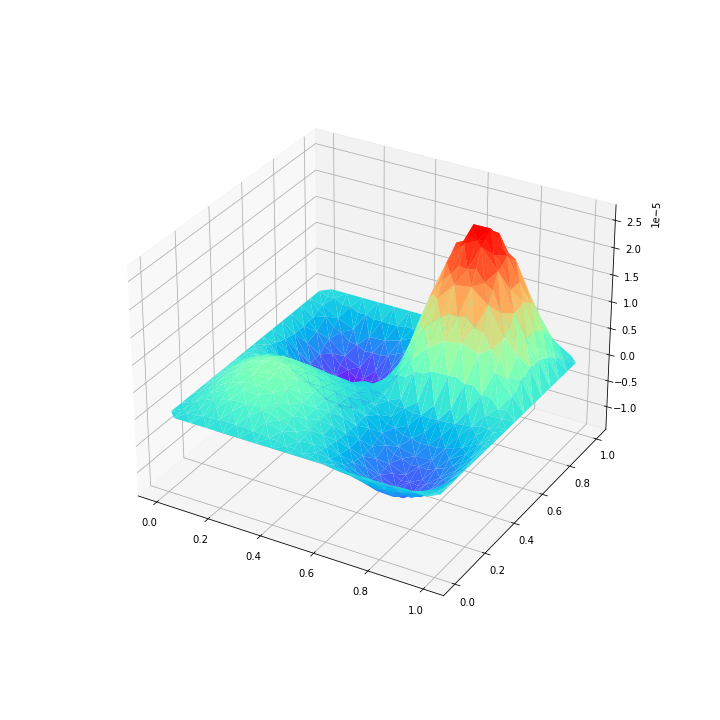
\includegraphics[height=5.7cm,width=5.7cm]{../image/interface_uh_u/interface2/uh_lam=[40000. 30000. 20000. 10000.].png}
			\label{interface2_uh_4}}	
		\subfigure[精确解图像]{
			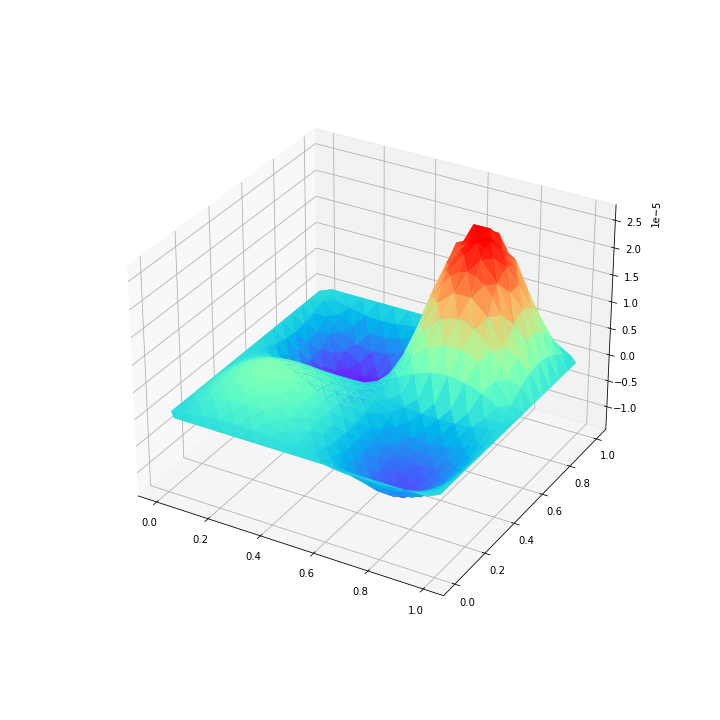
\includegraphics[height=5.7cm,width=5.7cm]{../image/interface_uh_u/interface2/u_lam=[40000. 30000. 20000. 10000.].png}
			\label{interface2_u_4}}
	\end{figure}
	
	\newpage
	
	\item 当Lam$\acute{e}$ 常数 $\lambda = \mu= [4E8,3E8,2E8,1E8]$ 时误差如下
	
	\begin{table}[h]
		\centering
		\caption{$|u-u_h|_{H^1(\Omega)}$}
		\scalebox{0.8}{
			\begin{tabular}{|c|c|c|c|c|} \hline
				h &0.5 &0.25 &0.125 &0.0625  \\ \hline
				$|u-u_h|_{H^1(\Omega)}$ &1.462698E-8 &6.166073E-9 &2.415138E-9 &2.373949E-9  \\ \hline
				H1误差阶 &1.246208 &0.532948 &0.819297 &0.939899 \\ \hline 
				$|u-u_h|_{L^2(\Omega)}$ &7.313491E-9 &1.541518E-9 &5.327030E-10 &1.509461E-10  \\ \hline
				L2误差阶 &2.246208 &1.532948 &1.819297 &1.939899 \\ \hline
		\end{tabular}}
	\end{table}
	
	\begin{figure}[h]
		\centering
		\caption{}
		\subfigure[数值解图像]{
			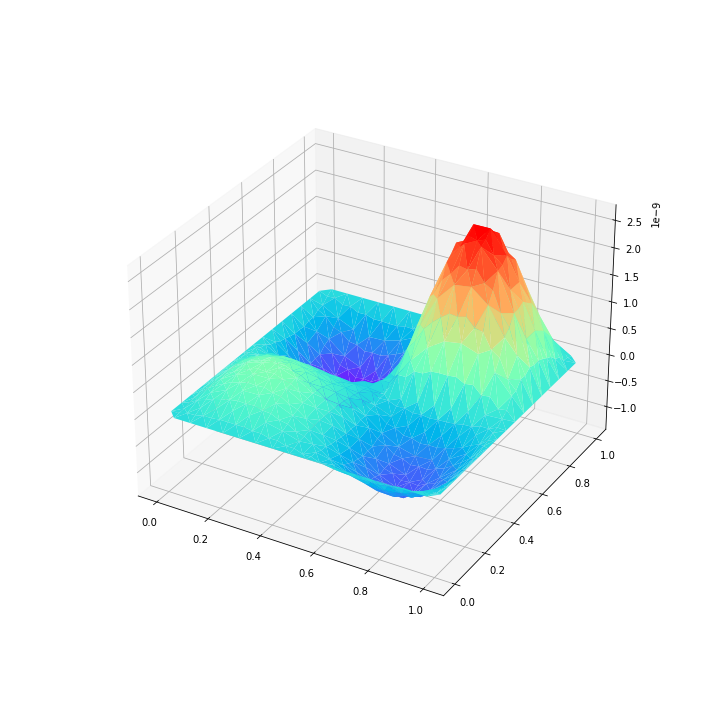
\includegraphics[height=5.7cm,width=5.7cm]{../image/interface_uh_u/interface2/uh_lam=[4.e+08 3.e+08 2.e+08 1.e+08].png}
			\label{interface2_uh_8}}	
		\subfigure[精确解图像]{
			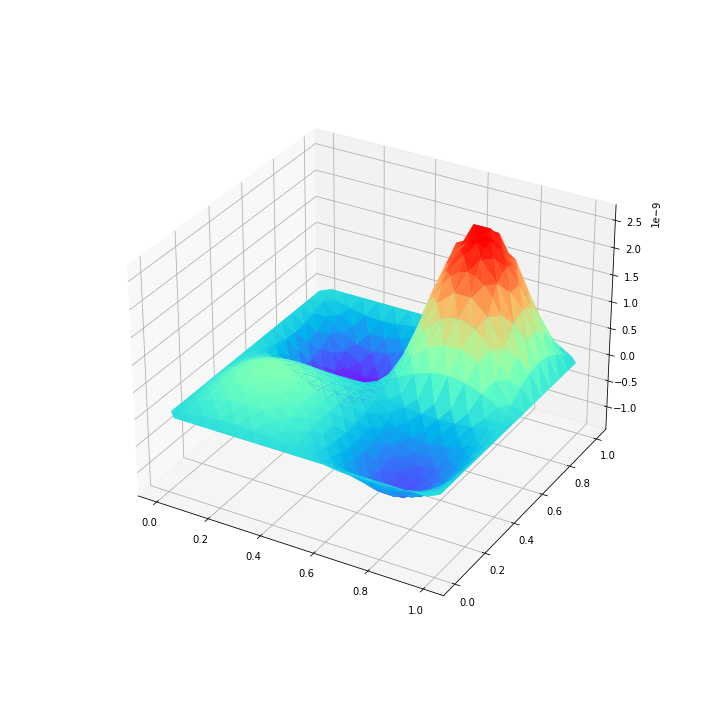
\includegraphics[height=5.7cm,width=5.7cm]{../image/interface_uh_u/interface2/u_lam=[4.e+08 3.e+08 2.e+08 1.e+08].png}
			\label{interface2_u_8}}
	\end{figure}
	
\end{enumerate}

\newpage

\section{总结}

本文使用 C-R 有限元方法求解了带间断系数的平面弹性问题,分析了非协调元对闭锁现象的影响。数值结果表明,当 Lam$\acute{e}$ 常数间断且相等时,C-R 元可以有效地解除闭锁现象,并且具有预期的收敛阶。

为了完善本文的研究,未来可以考虑对纯牵引力问题进行数值实验,以检验 C-R 元在不同的边界条件下的表现。同时,也可以通过改变间断系数的大小和形式,以及使用不同的网格划分方式,来进一步探究 C-R 元的有效性和稳定性,以及对间断系数的敏感性。

\newpage
\vfill

\CTEXsetup[format={\large\bfseries\songti\centering},beforeskip=0.5em,afterskip=0.5em]{section}
\bibliographystyle{unsrt}
\clearpage
\phantomsection
\addcontentsline{toc}{section}{参考文献}
\tolerance=500
\bibliography{interface_problem}

\newpage

%\chapter{\centerline{致谢}}
\section*{致谢}
\addcontentsline{toc}{section}{致谢}

时光荏苒, 岁月如梭, 转眼间大学生活来到了最后阶段. 当我写完这篇毕业论文的时候, 有一种如释重负的感觉, 感慨颇多. 回首大学四年, 得到过太多人的帮助了. 首先诚挚的感谢我的论文指导老师\textcolor{blue}{本科抽检}. 本文的研究工作都是在\textcolor{blue}{本科抽检}的悉心指导下完成的. \textcolor{blue}{本科抽检}平易近人, 严谨务实, 由于我知识储备不足, 在论文撰写过程中遇到了许多困难和疑惑, \textcolor{blue}{本科抽检}都及时给予指点, 耐心解释所犯的错误, 投入了大量的心血和精力, 更是不厌其烦地帮我察看论文中的小漏洞. \textcolor{blue}{本科抽检}对我的帮忙和关怀实在无法用言语表明. 还要感谢所有的老师们, 正是因为有了他们的督促和教导才能让我在这四年的学习生活里受益匪浅, 快速汲取专业知识, 提升专业能力. 同时也要感谢组内的同学们, 是他们以极大的热情来解答我在理论和程序上的疑问, 帮忙收集资料, 让平淡的日子不再那么枯燥乏味. 最后还要感谢我的家人, 是他们的支持与付出才给了我学习的机会, 感谢一直对我的理解, 这是我不断前进的动力. 

\iffalse
\newpage

\appendix
\section{附录 检测报告}

\begin{figure}[h]
	\centering
	
\includegraphics[height=16cm,width=13cm]{./push/1.png}
\end{figure}

\newpage

\begin{figure}[h]
	\centering
	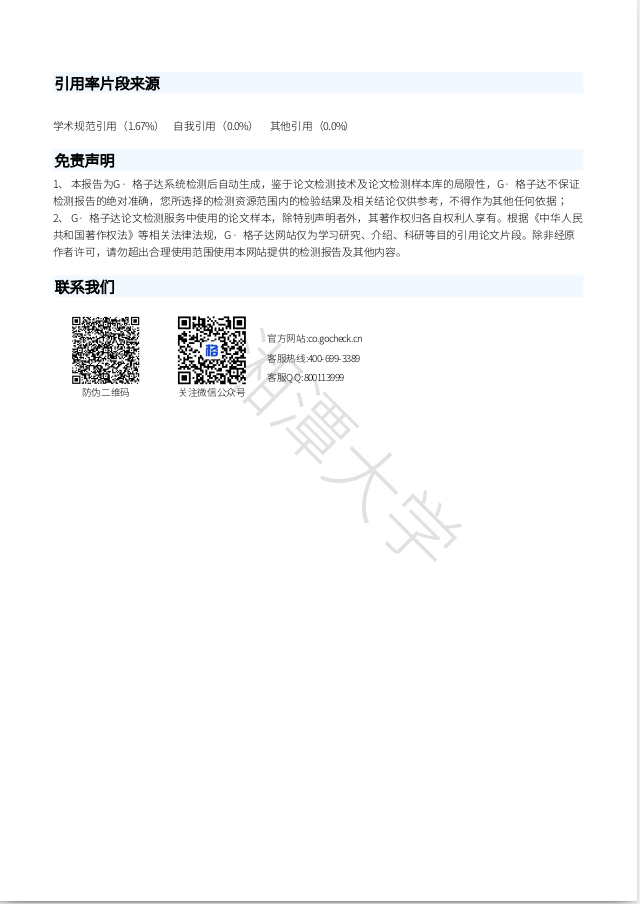
\includegraphics[height=16cm,width=13cm]{./push/2.png}
\end{figure}
\fi

\newpage
\appendix
\section{附录 数值程序}

\lstinputlisting[
style       =   Python,
caption     =   {\bf elasticityCR.py},
label       =   {elasticityCR.py}
]{../program/toPdf/interfaceCR.py}

\lstinputlisting[
style       =   Python,
caption     =   {\bf tool.py},
label       =   {tool.py}
]{../program/toPdf/tool.py}

\end{document}